\documentclass{article}

  % packages
    % basic stuff for rendering math
    \usepackage[letterpaper, top=1in, bottom=1in, left=1in, right=1in]{geometry}
    \usepackage[utf8]{inputenc}
    \usepackage[english]{babel}
    \usepackage{amsmath} 
    \usepackage{amssymb}
    % \usepackage{amsthm}

    % extra math symbols and utilities
    \usepackage{mathtools}        % for extra stuff like \coloneqq
    \usepackage{mathrsfs}         % for extra stuff like \mathsrc{}
    \usepackage{centernot}        % for the centernot arrow 
    \usepackage{bm}               % for better boldsymbol/mathbf 
    \usepackage{enumitem}         % better control over enumerate, itemize
    \usepackage{hyperref}         % for hypertext linking
    \usepackage{fancyvrb}          % for better lstlisting environments
    \usepackage{newverbs}         % for texttt{}
    \usepackage{xcolor}           % for colored text 
    \usepackage{listings}         % to include code
    \usepackage{lstautogobble}    % helper package for code
    \usepackage{parcolumns}       % for side by side columns for two column code
    

    % page layout
    \usepackage{fancyhdr}         % for headers and footers 
    \usepackage{lastpage}         % to include last page number in footer 
    \usepackage{parskip}          % for no indentation and space between paragraphs    
    \usepackage[T1]{fontenc}      % to include \textbackslash
    \usepackage{footnote}
    \usepackage{etoolbox}

    % for custom environments
    \usepackage{tcolorbox}        % for better colored boxes in custom environments
    \tcbuselibrary{breakable}     % to allow tcolorboxes to break across pages

    % figures
    \usepackage{pgfplots}
    \pgfplotsset{compat=1.18}
    \usepackage{float}            % for [H] figure placement
    \usepackage{tikz}
    \usepackage{tikz-dependency}
    \usepackage{tikz-cd}
    \usepackage{circuitikz}
    \usetikzlibrary{arrows}
    \usetikzlibrary{positioning}
    \usetikzlibrary{calc}
    \usepackage{graphicx}
    \usepackage{multirow}
    \usepackage{caption} 
    \usepackage{subcaption}
    \captionsetup{font=small}

    % for tabular stuff 
    \usepackage{dcolumn}

    \usepackage[nottoc]{tocbibind}
    \pdfsuppresswarningpagegroup=1
    \hfuzz=5.002pt                % ignore overfull hbox badness warnings below this limit

  % New and replaced operators
    \DeclareMathOperator{\Tr}{Tr}
    \DeclareMathOperator{\Sym}{Sym}
    \DeclareMathOperator{\Span}{span}
    \DeclareMathOperator{\std}{std}
    \DeclareMathOperator{\Cov}{Cov}
    \DeclareMathOperator{\Var}{Var}
    \DeclareMathOperator{\Corr}{Corr}
    \DeclareMathOperator{\pos}{pos}
    \DeclareMathOperator*{\argmin}{\arg\!\min}
    \DeclareMathOperator*{\argmax}{\arg\!\max}
    \newcommand{\ket}[1]{\ensuremath{\left|#1\right\rangle}}
    \newcommand{\bra}[1]{\ensuremath{\left\langle#1\right|}}
    \newcommand{\braket}[2]{\langle #1 | #2 \rangle}
    \newcommand{\qed}{\hfill$\blacksquare$}     % I like QED squares to be black

  % Custom Environments
    \newtcolorbox[auto counter, number within=section]{question}[1][]
    {
      colframe = orange!25,
      colback  = orange!10,
      coltitle = orange!20!black,  
      breakable, 
      title = \textbf{Question \thetcbcounter ~(#1)}
    }

    \newtcolorbox[auto counter, number within=section]{exercise}[1][]
    {
      colframe = teal!25,
      colback  = teal!10,
      coltitle = teal!20!black,  
      breakable, 
      title = \textbf{Exercise \thetcbcounter ~(#1)}
    }
    \newtcolorbox[auto counter, number within=section]{solution}[1][]
    {
      colframe = violet!25,
      colback  = violet!10,
      coltitle = violet!20!black,  
      breakable, 
      title = \textbf{Solution \thetcbcounter}
    }
    \newtcolorbox[auto counter, number within=section]{lemma}[1][]
    {
      colframe = red!25,
      colback  = red!10,
      coltitle = red!20!black,  
      breakable, 
      title = \textbf{Lemma \thetcbcounter ~(#1)}
    }
    \newtcolorbox[auto counter, number within=section]{theorem}[1][]
    {
      colframe = red!25,
      colback  = red!10,
      coltitle = red!20!black,  
      breakable, 
      title = \textbf{Theorem \thetcbcounter ~(#1)}
    } 
    \newtcolorbox[auto counter, number within=section]{proposition}[1][]
    {
      colframe = red!25,
      colback  = red!10,
      coltitle = red!20!black,  
      breakable, 
      title = \textbf{Proposition \thetcbcounter ~(#1)}
    } 
    \newtcolorbox[auto counter, number within=section]{corollary}[1][]
    {
      colframe = red!25,
      colback  = red!10,
      coltitle = red!20!black,  
      breakable, 
      title = \textbf{Corollary \thetcbcounter ~(#1)}
    } 
    \newtcolorbox[auto counter, number within=section]{proof}[1][]
    {
      colframe = orange!25,
      colback  = orange!10,
      coltitle = orange!20!black,  
      breakable, 
      title = \textbf{Proof. }
    } 
    \newtcolorbox[auto counter, number within=section]{definition}[1][]
    {
      colframe = yellow!25,
      colback  = yellow!10,
      coltitle = yellow!20!black,  
      breakable, 
      title = \textbf{Definition \thetcbcounter ~(#1)}
    } 
    \newtcolorbox[auto counter, number within=section]{example}[1][]
    {
      colframe = blue!25,
      colback  = blue!10,
      coltitle = blue!20!black,  
      breakable, 
      title = \textbf{Example \thetcbcounter ~(#1)}
    } 
    \newtcolorbox[auto counter, number within=section]{code}[1][]
    {
      colframe = green!25,
      colback  = green!10,
      coltitle = green!20!black,  
      breakable, 
      title = \textbf{Code \thetcbcounter ~(#1)}
    } 

    \BeforeBeginEnvironment{example}{\savenotes}
    \AfterEndEnvironment{example}{\spewnotes}
    \BeforeBeginEnvironment{lemma}{\savenotes}
    \AfterEndEnvironment{lemma}{\spewnotes}
    \BeforeBeginEnvironment{theorem}{\savenotes}
    \AfterEndEnvironment{theorem}{\spewnotes}
    \BeforeBeginEnvironment{corollary}{\savenotes}
    \AfterEndEnvironment{corollary}{\spewnotes}
    \BeforeBeginEnvironment{proposition}{\savenotes}
    \AfterEndEnvironment{proposition}{\spewnotes}
    \BeforeBeginEnvironment{definition}{\savenotes}
    \AfterEndEnvironment{definition}{\spewnotes}
    \BeforeBeginEnvironment{exercise}{\savenotes}
    \AfterEndEnvironment{exercise}{\spewnotes}
    \BeforeBeginEnvironment{proof}{\savenotes}
    \AfterEndEnvironment{proof}{\spewnotes}
    \BeforeBeginEnvironment{solution}{\savenotes}
    \AfterEndEnvironment{solution}{\spewnotes}
    \BeforeBeginEnvironment{question}{\savenotes}
    \AfterEndEnvironment{question}{\spewnotes}
    \BeforeBeginEnvironment{code}{\savenotes}
    \AfterEndEnvironment{code}{\spewnotes}

    \definecolor{dkgreen}{rgb}{0,0.6,0}
    \definecolor{gray}{rgb}{0.5,0.5,0.5}
    \definecolor{mauve}{rgb}{0.58,0,0.82}
    \definecolor{lightgray}{gray}{0.93}

    % default options for listings (for code)
    \lstset{
      autogobble,
      frame=ltbr,
      language=C,                           % the language of the code
      aboveskip=3mm,
      belowskip=3mm,
      showstringspaces=false,
      columns=fullflexible,
      keepspaces=true,
      basicstyle={\small\ttfamily},
      numbers=left,
      firstnumber=1,                        % start line number at 1
      numberstyle=\tiny\color{gray},
      keywordstyle=\color{blue},
      commentstyle=\color{dkgreen},
      stringstyle=\color{mauve},
      backgroundcolor=\color{lightgray}, 
      breaklines=true,                      % break lines
      breakatwhitespace=true,
      tabsize=3, 
      xleftmargin=2em, 
      framexleftmargin=1.5em, 
      stepnumber=1
    }

  % Page style
    \pagestyle{fancy}
    \fancyhead[L]{Natural Language Processing}
    \fancyhead[C]{Muchang Bahng}
    \fancyhead[R]{Spring 2024} 
    \fancyfoot[C]{\thepage / \pageref{LastPage}}
    \renewcommand{\footrulewidth}{0.4pt}          % the footer line should be 0.4pt wide
    \renewcommand{\thispagestyle}[1]{}  % needed to include headers in title page

\begin{document}

\title{Natural Language Processing}
\author{Muchang Bahng}
\date{Spring 2024}

\maketitle
\tableofcontents
\pagebreak

We will use NLTK, PyTorch. Natural language processing refers to the use of machine learning to learn language tasks. The problems are very broad and wide, including: 
\begin{enumerate}
  \item predictive typing 
  \item speech recognition 
  \item handwriting recognition 
  \item spelling/grammar correction 
  \item authorship identification 
  \item machine translation 
  \item summarization 
  \item dialogue 
  \item etc. 
\end{enumerate}
Obviously these are not simply just the ``ChatGPT"-like tasks that we are familiar with today, but use ideas from computer vision and other fields to develop better models. At the basis of a lot of these problems is \textbf{language modelling}, which will be the bulk of these notes. 

\section{Basics}

  \subsection{Regular Expressions}

    Regular expressions allow us to find patterns in strings. In Python, the $\texttt{r}$ in front of the string stands for \textbf{raw strings}, which literally takes in special characters (e.g. escape characters). Below, we search for the string $\texttt{and}$. 

    \begin{lstlisting} 
      import re 

      data = """Natural Language Processing (NLP) is an interdisciplinary field that empowers 
      67 machines to understand, interpret, and generate human language. Its 4 applications 
      span across various domains, including chatbots, language translation, sentiment 
      analysis, and information extraction. We're going to rock'n'roll in the long-term. """ 

      pattern = re.compile(r"and")
      matches = pattern.finditer(data) 

      for match in matches: 
          print(match) 
          
      # <re.Match object; span=(100, 103), match='and'>
      # <re.Match object; span=(116, 119), match='and'>
      # <re.Match object; span=(255, 258), match='and'>

      print(data[100:103], data[116:119], data[255:258])
      # and and and
    \end{lstlisting}

    There are special characters that allows us to identify other more specific patterns. We list them below. 
    \begin{lstlisting}
        .       - Any Character Except New Line
        \d      - Digit (0-9)
        \D      - Not a Digit (0-9)
        \w      - Word Character (a-z, A-Z, 0-9, _)
        \W      - Not a Word Character
        \s      - Whitespace (space, tab, newline)
        \S      - Not Whitespace (space, tab, newline)
        
        \b      - Word Boundary
        \B      - Not a Word Boundary
        ^       - Beginning of a String
        $       - End of a String
        
        []      - Matches Characters in brackets
        [^ ]    - Matches Characters NOT in brackets
        |       - Either Or
        ( )     - Group
    \end{lstlisting}

  \subsection{Preprocessing}

    \subsubsection{Tokenization and Stop Words}

      \textbf{Tokenization} is the process of dividing up a corpus or a complex sentence into words, also known as tokens. Using a streamlined series of regular expression evaluation, we are able to detect various words to tokenize. Note the following facts: 
      \begin{enumerate}
        \item Uppercase and lowercase versions of the same word (e.g. $\texttt{Language}$ vs $\texttt{language}$) are two different tokens. 
        \item Punctuations and special characters also count as a token (e.g. $\texttt{.}$, $\texttt{,}$, $\texttt{(}$, $\texttt{)}$). 
        \item Hyphenated words and some words with apostrophes are not separated, even though both components are valid words, since they are meant to be used together (e.g. $\texttt{rock'n'roll}$ or $\texttt{long-term}$). 
        \item Some words with apostrophes that are abbreviations are indeed separated (e.g. $\texttt{We're}$ to $\texttt{We}$, $\texttt{'re}$). 
      \end{enumerate}

      \begin{lstlisting}
        from nltk.tokenize import sent\_tokenize, word\_tokenize 

        example_string = """Natural Language Processing (NLP) is an interdisciplinary 
        field that empowers machines to understand, interpret, and generate human 
        language. Its applications span across various domains, including chatbots, 
        language translation, sentiment analysis, and information extraction. We're 
        going to rock'n'roll in the long-term. """


        print(sent\_tokenize(example_string))
        ['Natural Language Processing (NLP) is an interdisciplinary field that empowers 
        machines to understand, interpret, and generate human language.', 'Its 
        applications span across various domains, including chatbots, language 
        translation, sentiment analysis, and information extraction.', "We're going to 
        rock'n'roll in the long-term."]

        print(word_tokenize(example\_string))
        ['Natural', 'Language', 'Processing', '(', 'NLP', ')', 'is', 'an', 
        'interdisciplinary', 'field', 'that', 'empowers', 'machines', 'to', 
        'understand', ',', 'interpret', ',', 'and', 'generate', 'human', 'language', 
        '.', 'Its', 'applications', 'span', 'across', 'various', 'domains', ',', 
        'including', 'chatbots', ',', 'language', 'translation', ',', 'sentiment', 
        'analysis', ',', 'and', 'information', 'extraction', '.', 'We', "'re", 
        'going', 'to', "rock'n'roll", 'in', 'the', 'long-term', '.']
        0.004939079284667969 seconds 
      \end{lstlisting}

      Sometimes, there are words that are used so often that it is pointless to have them (e.g. $\texttt{the}$, $\texttt{an}$, $\texttt{a}$, etc.). We don't want these words to take up space in our database, so we can use NLTK to store a list of words that we consider to be stop words. The default library of \textbf{stop words} in multiple languages can be downloaded with the following command, and we can execute them on the paragraph above. In NLTK 3.8.1, there are a total of 179 stop words in English, and you can add or remove the words in this file manually. 

      \begin{lstlisting}
        nltk.download("stopwords") 
        from nltk.corpus import stopwords 

        print(stopwords.words("english"))

        ['i', 'me', 'my', 'myself', 'we', 'our', 'ours', 'ourselves', 'you', "you're", 
        "you've", "you'll", "you'd", 'your', 'yours', 'yourself', 'yourselves', 'he', 
        'him', 'his', 'himself', 'she', "she's", 'her', 'hers', 'herself', 'it', "it's", 
        ...
        'haven', "haven't", 'isn', "isn't", 'ma', 'mightn', "mightn't", 'mustn', 
        "mustn't", 'needn', "needn't", 'shan', "shan't", 'shouldn', "shouldn't", 'wasn', 
        "wasn't", 'weren', "weren't", 'won', "won't", 'wouldn', "wouldn't"]
      \end{lstlisting}

      To filter the stopwords, we can loop over the words in the token list and remove it if it is a stop word. 

    \subsubsection{Lemmatization and Stemming}

      \textbf{Stemming} is the process of producing morphological variants of a root word. For example, a stemming algorithm reduces the words ``chocolates", ``chocolatey", and ``choco" to the root word ``chocolate." It helps to reduce different variants into a unified word for easier retrival of data. 

      \begin{lstlisting}
        from nltk.stem import PorterStemmer 

        ps = PorterStemmer() 
        words = ["program", "programs", "programmer", "programming", "programmers"]
        for w in words:
            print(w, " : ", ps.stem(w))

         program  :  program
         programs  :  program
         programmer  :  program
         programming  :  program
         programmers  :  program
      \end{lstlisting}

  \subsection{Syntactic Structure}

    \subsubsection{Parts of Speech}

      The parts of speech can be defined with varying degrees of refinement. First, let us get the basics down. Parts of speech fall into two broad categories: \textbf{closed class} and \textbf{open class}. Closed classes are those with relatively fixed membership, such as prepositions (new prepositions are rarely coined). However, nouns and verbs are open class since new nouns and verbs (e.g. iPhone or to fax) are always being created. 

      \begin{table}[H]
        \centering
        \small
        \begin{tabular}{|c|l|p{8cm}|>{\itshape}p{4.5cm}|}
        \hline
        \textbf{Class} & \textbf{Tag} & \textbf{Description} & \textbf{Example} \\
        \hline
        \multirow{6}{*}{\rotatebox[origin=c]{90}{Open Class}} & ADJ & Adjective: noun modifiers describing properties & red, young, awesome\\
        & ADV & Adverb: verb modifiers of time, place, manner & very, slowly, home, yesterday \\
        & NOUN & Words for persons, places, things, etc. & algorithm, cat, mango, beauty \\
        & VERB & Words for actions and processes & draw, provide, go \\
        & PROPN & Proper noun: name of a person, organization, place, etc. & Regina, IBM, Colorado \\
        & INTJ & Interjection: exclamation, greeting, yes/no response, etc. & oh, um, yes, hello \\
        \hline
        \multirow{8}{*}{\rotatebox[origin=c]{90}{Closed Class}} & ADP & Adposition (Preposition/Postposition): marks a noun’s spatial, temporal, or other relation & in, on, by, under \\
        & AUX & Auxiliary: helping verb marking tense, aspect, mood, etc. & can, may, should, are \\
        & CCONJ & Coordinating Conjunction: joins two phrases/clauses & and, or, but \\
        & DET & Determiner: marks noun phrase properties & a, an, the, this \\
        & NUM & Numeral & one, two, first, second \\
        & PART & Particle: a function word that must be associated with another word & 's, not, (infinitive) to \\
        & PRON & Pronoun: a shorthand for referring to an entity or event & she, who, I, others \\
        & SCONJ & Subordinating Conjunction: joins a main clause with a subordinate clause such as a sentential complement & that, which \\
        \hline
        \multirow{3}{*}{\rotatebox[origin=c]{90}{Other}} & PUNCT & Punctuation & ; , () \\
        & SYM & Symbols like \$ or emoji & \$, \% \\
        & X & Other & asdf, qwfg \\
        \hline
        \end{tabular}
        \caption{Class, Tag, Description, and Example}
        \label{table:class_tag_description_example}
      \end{table}

      Now there are two prominent frameworks used in the field of syntax to describe the structure of sentences in natural languages: \textbf{Phrase Structure Grammar (PSG)} and \textbf{Dependency Grammar (DG)}. They differ in their underlying principles, so we will introduce them separately. 

    \subsubsection{Phrase Structure/Context Free Grammar}

      We have our starting units as words
      \begin{lstlisting}
        the     cat    cuddly    by     door 
        DET     NOUN   ADJ       PREP   NOUN 
      \end{lstlisting}
      Now these words can combine into phrases. A \textbf{noun phrase} ($\texttt{NP}$) refers to a phrase describing a noun; a \textbf{verb phrase} ($\texttt{VP}$) refers to a phrase describing a verb, and a \textbf{prepositional phrase} ($\texttt{PP}$) refers to describing a noun's spatial, tempral, or other relation. 
      \begin{lstlisting}
        the cuddly cat     by [the door]    walking over there 
        NP                 PP  NP           VP 
      \end{lstlisting}
      From the example above, we can see that these phrases can be nested within each other. For example, 
      \begin{lstlisting}
          the cuddly cat by the door 
          [     NP     ]    [  NP  ]
                         [    PP   ]
          [           NP           ]
      \end{lstlisting}
      We can make rules for how NP, PP and VPs are structured. By looking at $\texttt{the cuddly cat}$, we can make the following rule 
      \begin{lstlisting}
          NP --> DET ADJ NOUN
      \end{lstlisting}
      The adjective can be there or not, so in linguistics we have the notation $\texttt{(ADJ)*}$. Furthermore, if we attach a prepositional phrase at the end, we can have some structure like 
      \begin{lstlisting}
          NP --> DET (ADJ)* NOUN (PP)
      \end{lstlisting}
      which is a generalization of the first rule. A prepositional phrase such as $\texttt{by the door}$ has the structure 
      \begin{lstlisting}
          PP --> PREP DET NOUN
      \end{lstlisting}
      A verb phrase like $\texttt{talked to the cat}$ has the structure 
      \begin{lstlisting}
          VP --> VERB PREP DET NOUN
      \end{lstlisting}
      These set of rules is called the \textbf{grammar}, and they determine what phrases we are or aren't allowed to use. If we have another phrase like $\texttt{the cat walked behind the dog}$, which is a valid sentence, we need to account for this validity by adding the extra grammar rules 
      \begin{lstlisting}
          the  cat  walked  behind  the  dog 
          [  NP  ] [          VP          ]
          [  NP  ] [ VERB]  [      PP     ]
          DET  NOUN VERB    PREP    DET  NOUN 
      \end{lstlisting}
      But there are a countless variety of sentences out there, and we can't keep making rules forever. 

    \subsubsection{Dependency Grammar}

      While phrase structure grammar is a popular paradigm for syntax construction, starting from the early 2000s, NLP researchers have swung behind dependency grammar. Given a phrase or a sentence, the \textbf{dependency structure} shows which words depend on (modify, attach to, or are arguments of) which other words. Humans communicate complex ideas by composing words together into bigger units to convey complex meanings. Listeners need to work out what modifies what, and similarly, a model needs to understand sentence structure in order to be able to interpret language correctly. 

      Let us start off with understanding what it means for a word to be dependent on another. Informally, a word A is a dependent of word B if B is needed to complete the phrase of A. 

      The basic idea is given a sentence, we want to take each word and find out its part of speech and what other words modify it. This creates a \textbf{dependency tree}. 

      \begin{center}
        \begin{dependency}[theme = simple]
        \begin{deptext}[column sep=1em]
        Look \& in \& the \& large \& crate \& in \& the \& kitchen \& by \& the \& door \\
        \end{deptext}
        \deproot{1}{}
        \depedge{5}{3}{} 
        \depedge{5}{4}{}
        \depedge{8}{7}{}
        \depedge{11}{10}{}
        \depedge{1}{5}{}
        \depedge{8}{6}{}
        \depedge{11}{9}{}
        \depedge{5}{2}{}
        \depedge{5}{11}{}
        \depedge{5}{8}{}
        \end{dependency}
      \end{center}

      The dependency structure answers questions like ``which crate?" or ``where are you looking?" It may be more natural for us to have $\texttt{in}$ as a dependency of $\texttt{look}$, with $\texttt{crate}$ being the dependency of of $\texttt{in}$, as such 

      \begin{center}
        \begin{dependency}[theme = simple]
        \begin{deptext}[column sep=1em]
        Look \& in \& the \& large \& crate \\
        \end{deptext}
        \deproot{1}{}
        \depedge{1}{2}{}
        \depedge{2}{5}{}
        \depedge{5}{3}{}
        \depedge{5}{4}{}
        \end{dependency}
      \end{center}

      However, in the \textbf{universal dependency structure}, which aims to create these for many human languages, the design decisions led to the other convention. 

      Dependency structure is especially important to minimize ambiguity, as in the following phrases: 
      \begin{enumerate}
        \item \textit{Prepositional Phrase Attachment Ambiguity: } The sentence can have two meanings: The police in San Jose kill a man who has a knife, or the police in San Jose use a knife to kill a man. 

        \begin{center}
        \begin{dependency}[theme = simple]
        \begin{deptext}[column sep=1em]
        San \& Jose \& cops \& kill \& man \& with \& knife \\
        \end{deptext}
        \deproot{4}{}
        \depedge{3}{1}{}
        \depedge{3}{2}{}
        \depedge{4}{3}{}
        \depedge{4}{5}{}
        \depedge{5}{7}{}
        
        \deproot[edge below]{4}{}
        \depedge[edge below]{3}{1}{}
        \depedge[edge below]{3}{2}{}
        \depedge[edge below]{4}{3}{}
        \depedge[edge below]{4}{5}{}
        \depedge[edge below]{4}{7}{}
        \end{dependency}
        \end{center}

        \item \textit{Coordination Scope Ambiguity}: We don't know whether Michael Jordan is both an NBA and MLB player, or if an NBA player is separate. 

        \begin{center}
        \begin{dependency}[theme = simple]
        \begin{deptext}[column sep=1em]
        NBA \& player \& and \& MLB \& player \& Michael \& Jordan \& appointed \& to \& board \\
        \end{deptext}
        \deproot{8}{}
        \depedge{2}{1}{}
        \depedge{6}{4}{}
        \depedge{6}{5}{}
        \depedge{2}{3}{}
        \depedge{2}{6}{}
        \depedge{7}{2}{}
        \depedge{8}{7}{}
        \depedge{8}{10}{}

        \depedge[edge below]{2}{1}{}
        \depedge[edge below]{7}{4}{}
        \depedge[edge below]{7}{5}{}
        \depedge[edge below]{7}{6}{}
        \depedge[edge below]{2}{3}{}
        \depedge[edge below]{2}{7}{}
        \depedge[edge below]{8}{2}{}
        \depedge[edge below]{8}{10}{}
        \end{dependency}
        \end{center}

        \item \textit{Verb Phrase Attachment Ambiguity}: For example, ``mutilated body washes up on Rio beach to be used for Olympics beach volleyball." 

        
        \item \textit{Adjective/Adverbial Modifier Ambiguity}
      \end{enumerate}

    \subsubsection{Dependency Conditioning Preferences}

      Now comparing these two paradigms, it may seem that writing a set of grammar rules may be more efficient than using a collection of dependency trees, called \textbf{tree banks}. After all, having a set of general grammar rules certainly seems easier than getting people to annotate a bunch of text with their parts of speech and modifiers. But treebanks are good since we can reuse the labor (many parsers and parts-of-speech taggers can be built on top of it), it gives broad coverage and not just a few intuitions, and it gives frequencies and distributional information of these words. Furthermore, there are other more useful sources of information: 
      \begin{enumerate}
        \item \textit{Bilexial affinities}: The dependency is plausible 
        \item D\textit{ependency Distance}: Most dependencies are between nearby words. 
        \item \textit{Intervening Material}: Dependencies rarely span intervening words or punctuation. 
        \item \textit{Valency of Heads}: How many dependents on which side are usual for a head? e.g. given a noun, what kind of dependents would it have usually? It would normally have a determiner to the left (and almost never to the right) and an adjective to the left also. Perhaps a verb to the right. 
      \end{enumerate}

      Furthermore, there are some constraints on these dependencies, such as only one word is a dependent of ROOT and we don't want any cycles. This makes dependencies a tree, hence the name. The final issue is whether arrows can cross (be non-projective) or not. The definition of a \textbf{projective parse} is that there are no crossing dependency arcs when the arrows are laid out in their linear order, which all arcs above the words. Usually, we want the arrows to be projective so that we have a nested phrase structure like we saw in context free grammar, and most syntactic structure is projective, but dependency theory normally does allow non-projective structures to account for displaced constituents. 

      Now as for building dependency parsers, there are many ways to do this: 
      \begin{enumerate}
        \item \textit{Dynamic Programming} (Eisner 1996) gives a clever algorithm with complexity $O(n^3)$ by producing parse items with heads at the ends rather than in the middle. 
        \item \textit{Graph Algorithms}: You create a minimum spanning tree for a sentence. 
        \item \textit{Constraint Satisfaction}: Edges are eliminated that don't satisfy hard constraints. 
        \item \textit{Transition-Based Parsing} or \textit{Deterministic Dependency Parsing} uses a greedy choice of attachments guided by good machine learning classifiers. 
      \end{enumerate}

\section{Embeddings}

    Our goal is to create some embedding method that maps the vocabulary of words into some vector space $\mathbf{V}$. One could simply one-hot-encode all the words, but this is memory inefficient and the structure of the words are not captured. That is, we would like some associated metric $d$ that tells us how similar two words are. At this point, it is not clear that this similarity entails, whether it'd be similar definitions (dog and canine), similar in groupings (e.g. dog and cat), or similar in context (doctor and scalpel). 

    There have been many attempts to create this mapping, but the most successful by far has followed the idea of \textbf{distributional semantics}. This hypothesis states that words that occur in similar contexts tend to have similar meanings. 

  \subsection{Frequency Semantics}

    \subsubsection{Term-Document Matrix}

      Let's start with the simplest distributional model based on the \textbf{co-occurence matrix}, which represents how often words co-occur. 

      \begin{definition}[Term-Document Matrix]
        Given $\mathcal{D} = \{D_1, \ldots, D_m\}$ documents and $\mathcal{V} = \{v_1, \ldots, v_n\}$ total words (tokens) in the document, the \textbf{term-document matrix} is a $n \times m$ matrix where the $ij$th entry represents the number of times token $v_i$ occurred in document $D_j$. One can see how this will be a sparse matrix, since there may be many infrequent words that appear only once in exactly one document. 
      \end{definition}

      \begin{example}
        Given the following three documents 
        \begin{align*}
            D_1 & : \texttt{I like deep learning. } \\
            D_2 & : \texttt{I like NLP. } \\
            D_3 & : \texttt{I enjoy flying.}
        \end{align*}
        we can construct a term-document matrix as 
        \begin{table}[H]
          \centering
          \begin{tabular}{|c||*{3}{c|}}
          \hline
           & $D_1$ & $D_2$ & $D_3$ \\ 
          \hline\hline
          I       & 1 & 1 & 1 \\ \hline
          like    & 1 & 1 & 0\\ \hline
          deep    & 1 & 0 & 0 \\ \hline
          learning& 1 & 0 & 0 \\ \hline
          NLP     & 0 & 1 & 0 \\ \hline
          enjoy   & 0 & 0 & 1 \\ \hline
          flying  & 0 & 0 & 1 \\ \hline
          \end{tabular}
          \caption{Term-Document Matrix}
        \end{table}
      \end{example}

      Now there are two ways that we can analyze this matrix. First, note that the columns $M_{:, i}$ are vectors that represent the words in document $D_i$. This is known as the \textbf{bag-of-words model}. The rows $M_{j, :}$ represent the frequency of a certain word $v_j$ in each document. Therefore, we can compare documents by comparing their corresponding vectors $D_i, D_j$ which represent the distribution of its words, and we can compare words by comparing their corresponding vectors $v_i, v_j$, which represent their distribution over the documents. 

      Upon inspection you can notice that this is exactly feature extraction. Each document in the corpus is a data point and the count of specific words are the features. We can implement this with scikit learn's feature extractor, which gives the word count of a corpus, represented as a list of strings. We first load in our corpus. 
      \begin{lstlisting}
        from sklearn.feature_extraction.text import CountVectorizer
        import pandas as pd

        corpus = [
            "I like deep learning.", 
            "I like NLP.", 
            "I enjoy flying."
        ]

        cvectorizer = CountVectorizer()
        X = cvectorizer.fit_transform(corpus)
        terms = cvectorizer.get_feature_names_out()

        # List of all terms in order of document-term matrix columns. 
        print(terms)
        # ['deep' 'enjoy' 'flying' 'learning' 'like' 'nlp']

        # Document term matrix 
        print(X.toarray())
        # [[1 0 0 1 1 0]
        #  [0 0 0 0 1 1]
        #  [0 1 1 0 0 0]]

        # Data type of matrix and shape (note this is a sparse matrix type) 
        print(type(X))      # <class 'scipy.sparse._csr.csr_matrix'> 
        print(X.shape)      # (3, 6) 

        documentTermMatrix = pd.DataFrame(X.toarray(),
                                          index=["Doc 1", "Doc 2", "Doc 3", ],
                                          columns=terms)

        print(documentTermMatrix.to_string())

               deep  enjoy  flying  learning  like  nlp
        Doc 1     1      0       0         1     1    0
        Doc 2     0      0       0         0     1    1
        Doc 3     0      1       1         0     0    0
      \end{lstlisting}

    \subsubsection{Term-Term Matrix}

      Another way to compare words is through a term-term matrix. 

      \begin{definition}[Term-Term Matrix]
        A \textbf{term-term matrix}, or a \textbf{co-occurence matrix}, is a $|V| \times |V|$ matrix that represents the number of times the row (target, center) word and the column (context) word co-occur in some context in some training corpus. 
        \begin{enumerate}
          \item The context could be the document, in which case the element $M_{ij}$ represents the number of times the two words $v_i, v_j$ appear in the same document. 
          \item It is most common to use smaller contexts, generally a window around the word, e.g. $\pm 4$ words, in which case $M_{ij}$ represents the number of times (in some training corpus) $v_j$ appears around $\pm 4$ words around $v_i$. 
        \end{enumerate}
      \end{definition}

      \begin{example}
        Given a window length of $1$ (most common for window length to be 5 through 10) and a corpus of three documents: 
        \begin{align*}
            D_1 & : \texttt{I like deep learning. } \\
            D_2 & : \texttt{I like NLP. } \\
            D_3 & : \texttt{I enjoy flying.}
        \end{align*}
        the co-occurence matrix (note that it should be symmetric). is 
        \begin{table}[H]
        \centering
        \begin{tabular}{|c||*{7}{c|}}
        \hline
         & I & like & deep & learning & NLP & enjoy & flying \\ 
        \hline\hline
        I       & 0 & 2 & 1 & 0 & 0 & 1 & 0 \\ \hline
        like    & 2 & 0 & 1 & 0 & 1 & 0 & 0 \\ \hline
        deep    & 1 & 1 & 0 & 1 & 0 & 0 & 0 \\ \hline
        learning& 0 & 0 & 1 & 0 & 0 & 0 & 0 \\ \hline
        NLP     & 0 & 1 & 0 & 0 & 0 & 0 & 0 \\ \hline
        enjoy   & 1 & 0 & 0 & 0 & 0 & 0 & 1 \\ \hline
        flying  & 0 & 0 & 0 & 0 & 0 & 1 & 0 \\ \hline
        \end{tabular}
        \caption{Co-occurrence Matrix}
        \end{table}
      \end{example}

      This gives us a representation of words as \textbf{co-occurence vectors}, which is similar to the word2vec embedding since they both use windows of a certain size. 

  \subsection{Cosine Similarity}

    To measure similarity between two words or documents, it may be natural to take some sort of distance in $\mathbb{R}^{|V|}$. However, due to the size of the documents being nonuniform, we would like to measure how parallel one vector is to another. Two very similar documents $D_i, D_j$, where one is twice as long as the other, would be expected to have a proportional document vector satisfying $D_i \approx 2 D_j$. Therefore, the angle between the two vectors would be best representation of the similarity metric. 

    \[\mathrm{cosine}(v_i, v_j) = \frac{v_i \cdot v_j}{||v_i|| \, ||v_j||} = \cos{\theta}\]

  \subsection{TF-IDF and PMI}

    Let us focus on the vectors representing words, where the dimensions are documents. The words $v_1, v_2$ are essentially defined by their frequency in a corpus of documents $D_1, \ldots, D_m$. The TF-IDF algorithm focuses on two main modifications of the frequency representation mentioned above. 
    \begin{enumerate}
      \item \textit{TF}: The raw frequency of the words may be a skewed representation of the token, since the difference between $0$ and $1$ occurrence in document $D_i$ is not the same as the difference between $1000$ and $1001$ occurrences in another document. Unimportant stop words like ``the" that occur frequently enough shouldn't have as much of an effect on the representation of the word. We can filter these stop words out like before, but depending on context, there may be other words that are a less drastic impact. The additional impact of another instance of a word should have diminishing returns. 
      \item \textit{IDF}: ``Special" words that occur in only a few documents should have higher weights, since they are useful for discriminating those documents from the rest of the collection. Therefore, we would want this measure to be inversely proportional to the number of documents it is in. We can define 
      \[\frac{N}{\mathrm{df}_t}\]
      where $N$ is the total number of documents and $\mathrm{df}_t$ is the number of documents that word $t$ is in. Due to the large number of documents in a corpus, this value is also squashed down by a logarithm. 
    \end{enumerate}
    Given these two ideas, we define the two following forms of measure. 

    \begin{definition}[TF]
      The \textbf{term frequency} is a measure of the frequency of the word $t$ in the document $d$, squashed by the logarithm function (by diminishing returns) and adding $1$ so that this weight is $0$ when there are $0$ occurences. 
      \[\mathrm{tf}_{t, d} = \log_{10} \big( \mathrm{count}(t, d) + 1 \big)\]
    \end{definition}

    \begin{definition}[IDF]
      The \textbf{inverse document frequency} is defined 
      \[\mathrm{idf}_t = \log_{10} \bigg( \frac{N}{\mathrm{df}_t} \bigg)\]
    \end{definition}

    \begin{definition}[tf-idf]
      The \textbf{tf-idf} weighted value for word $t$ in document $d$ thus combines the two values together. 
      \[w_{t, d} \coloneqq \mathrm{tf}_{t, d} \cdot \mathrm{idf}_{t}\]
    \end{definition}

    You can implement this in sklearn with the Tf-idf vectorizer, which again extracts features from a corpus. Let us use the same corpus as above. We can compare this matrix to the document-term matrix. 
    \begin{lstlisting}
      from sklearn.feature_extraction.text import TfidfVectorizer
      import pandas as pd

      corpus = [
          "I like deep learning.", 
          "I like NLP.", 
          "I enjoy flying."
      ]

      vectorizer = TfidfVectorizer() 
      X = vectorizer.fit_transform(corpus)

      tfidfMatrix = pd.DataFrame(X.toarray(),
                                  index=["Doc 1", "Doc 2", "Doc 3", ],
                                  columns=terms)

      print(tfidfMatrix)
                 deep     enjoy    flying  learning      like       nlp
      Doc 1  0.622766  0.000000  0.000000  0.622766  0.473630  0.000000
      Doc 2  0.000000  0.000000  0.000000  0.000000  0.605349  0.795961
      Doc 3  0.000000  0.707107  0.707107  0.000000  0.000000  0.000000
    \end{lstlisting}

    An alternative weighting function to tf-idf is the PPMI (positive PMI), which is used for term-term matrices, when the vector dimensions correspond to words rather than documents. PPMI draws on the intuition that the best way to weigh the association between two words is to ask how much more the two words co-occur in our corpus than we would have a priori expected to appear by chance. 

    \begin{definition}[PMI]
    The \textbf{pointwise mutual information} between a target word $w$ and context word $c$ is defined as
    \[\mathrm{PMI}(w, c) = \log_2 \frac{P (w, c)}{P(w)\, P(c)}\]
    We can see that the numerator observes the joint distribution of the two words observed together, while the denominator represents their observation independently. We take the logarithm so that its range is $(-\infty, +\infty)$, where a value of greater than $0$ indicates that the words co-occur more often and values less than $0$ indicates that words are co-occuring less often than chance. However, negative PMI values tend to be unreliable since these probabilities can get very small, unless our corpus is enormous. Therefore, in practicality, we use the \textbf{positive PMI}, which just sets all negative values to $0$. 
    \[\mathrm{PPMI}(w, c) = \max \bigg\{ 0, \log_2 \frac{P (w, c)}{P(w)\, P(c)} \bigg\}\]
    \end{definition}

    Given a term-term matrix, we can organize the PPMIs in a matrix. That is, let $f_{ij}$ be the number of times word $w_i$ occurs in context $c_j$. 

  \subsection{Latent Semantic Analysis (LSA)}

    Clearly, we can see that text data suffers from many problems. 
    \begin{enumerate}
      \item the vectors increase in size with vocabulary 
      \item it is very high dimensional and requires a lot of storage, though it is sparse. Even after preprocessing methods such as stop word removing, tokenization, and stemming, the document-term or TF-IDF matrices $\mathbf{A}$ are extremely high dimensional. 
      \item subsequent classification models have sparsity issues, implying that models may be less robust
    \end{enumerate}
    Our idea is to store the most important information in a fixed, small number of dimensions (ideally between 25 and 1000): a dense vector. A linear dimensionality reduction technique is to use principal component analysis. We basically take the SVD of the matrix, which reformulates the text data of $r$ linearly uncorrelated \textbf{latent (hidden) features} through a \textbf{low-rank approximation}. 

    There are multiple motivations for this: 
    \begin{enumerate}
      \item The original matrix may simply by too large to handle computationally and this approximation is a necessary evil. 
      \item The original matrix may be noisy, and anecdotal instances of terms are to be eliminated. 
      \item The original matrix may be overly sprase relative to the ``true" matrix. That is, the original matrix lists only the words actually in each document, whereas we may be interested in all words \textit{related} to each document. 
    \end{enumerate}
    We take the SVD of the matrix, 
    \[\mathbf{A} = \mathbf{U} \boldsymbol{\Sigma} \mathbf{V}^T\]
    where $\mathbf{U}$ and $\mathbf{V}$ are unitary, with $\boldsymbol{\Sigma}$ diagonal. By rearranging the columns of $\mathbf{U}$ and $\mathbf{V}$, we can have the diagonal entries (i.e. singular values) of $\boldsymbol{\Sigma}$ to go from greatest to least. Since the yellow part in the middle matrix is $0$, the yellow of the right does not matter in the decomposition. Now to perform dimensionality reduction, we can remove the blue parts. 
    \begin{center}
      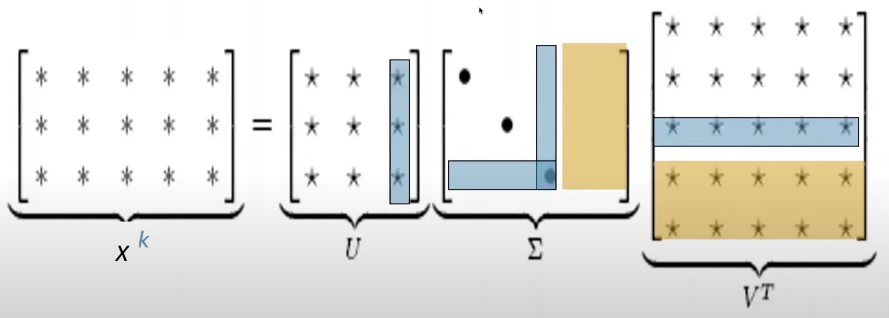
\includegraphics[scale=0.3]{img/SVD.png}
    \end{center}
    That is, we 
    \begin{enumerate}
      \item Keep the top $k$ right singular vectors $\mathbf{V} \mapsto \mathbf{V}_k$ 
      \item Keep the top $k$ left singular vectors $\mathbf{U} \mapsto \mathbf{U}_k$
      \item Keep only the top $k$ singular values $\boldsymbol{\Sigma} \mapsto \boldsymbol{\Sigma}_k$
    \end{enumerate}
    The rank-$k$ approximation is 
    \[\mathbf{A}_k = \mathbf{U}_k \boldsymbol{\Sigma}_k \mathbf{V}_k^T\]
    After this, the documents and the words are combard by cosine similarity. It turns out that the normal error assumptions for SVD does not align with the structure of the raw counts data, which may be skewed with extremely frequent words (e.g. ``the"). Therefore, we can focus on the TF-IDF matrix, which logs the frequencies, bounds some counts, or may ignore stop words. These kinds of models were explored a lot in the 90s or the 00s, with creative ideas like ramped windows that weighted closer words more than further ones, or used Pearson correlations instead of counts. In fact, Rohde's COALS model showed interesting semantic properties between words that captured nice patterns between an action and an individual doing the action. 
    \begin{center}
        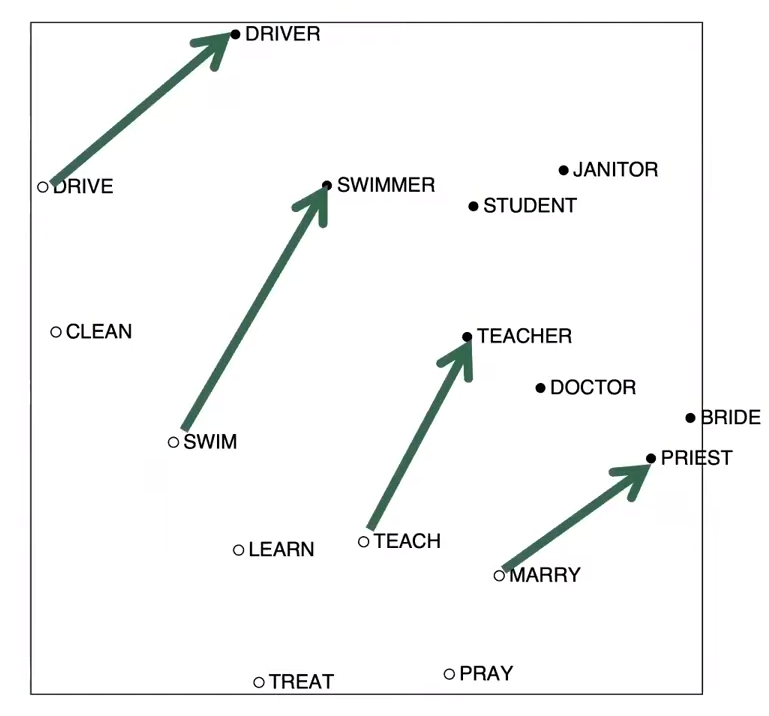
\includegraphics[scale=0.25]{img/COALS.png}
    \end{center}
    So by taking the vector differences we can say things like ``drive is to driver as swim is to swimmer." 

  \subsection{GenSim Package (Generate Similar)}

    The Python package gensim is used to implement the word2vec algorithm. The core concepts of the package are: 
    \begin{enumerate}
      \item \textit{Document}: Some text represented by a string. 
      \item \textit{Corpus}: A collection of documents. 
      \item \textit{Vector}: A mathematically convenient representation of a document. 
      \item \textit{Model}: An algorithm for transforming vectors from one representation to another. 
    \end{enumerate}

  \subsection{Word2Vec}

      Note that the word representations are sparse. There are many computational tricks to work with sparse vectors, but there tends to be lots of noise and problems with them. Rather, we look at a more powerful word representation called \textbf{embeddings}, which are short dense vectors ranging in dimension from $50$ to $1000$. It turns out that dense vectors work better in every NLP task than sparse vectors. 

      The intuition for word2vec is that instead of counting how often each word $w$ occurs near, say \textit{apricot}, we'll instead train a classifier on a binary prediction task: ``Is word $w$ likely to show up near \textit{apricot}?" We don't actually care about this prediction task. Intead, we will take the learned classifier weights as the word embeddings. Furthermore, we can just use running text as implicitly supervised training data. A context word $c$ that occurs near \textit{apricot} acts as a sample of ``yes" to the question above. 

      Imagine a sentence like the following, with \textbf{target word} \textit{apricot}, with a windows of $\pm2$ \textbf{context words}. 
      \[\texttt{... lemon, a [ tablespoon of apricot jam, a ] pinch ...}\]
      Now our goal is to train a classifier where given the pair $\mathbf{x} = (\mathbf{w}, \mathbf{c})$, our output must be $y \in \{0, 1\}$, where $0$ means not existing and $1$ means within. This means that $y \mid \mathbf{x} \sim \mathrm{Bernoulli}(\mu)$, where $\mu$ is dependent on $(\mathbf{w}, \mathbf{c})$. This probability should be higher the more similar $\mathbf{w}$ and $\mathbf{c}$ are. We have already established that the similarity metric can be effectively represented by the dot product, we have 
      \[\mu = \mu(\mathbf{w}, \mathbf{c}) = \frac{1}{1 + \exp(- \mathbf{w} \cdot \mathbf{c})}\]
      and so, the idea of our algorithm is that every time we find a window of context words around a target word, we should update both $\mathbf{w}$ and $\mathbf{c}$ s.t. they are more parallel. 

    \subsubsection{Skip Gram with Negative Sampling}

      Let us formalize this concept a bit. Let us one-hot encode every word in our corpus to the set 
      \[\mathcal{V} = \{\mathbf{v}_1, \ldots, \mathbf{v}_{|\mathcal{V}|}\}\] 
      Now, what we wish to do is to embed all these vectors in some $\mathbb{R}^E$, where $E$ is a hyperparameter that we select and preferably $E < |\mathcal{V}|$. The embeddings $\mathbf{w}_i$ for every $\mathbf{v}_i = \mathbf{e}_i$ can be simply stored as the columns of a $E \times |V|$ matrix. 
      \[\begin{pmatrix} | & \ldots & | \\ \mathbf{w}_1 & \ldots & \mathbf{w}_{|\mathcal{V}|} \\ | & \ldots & | \end{pmatrix} \begin{pmatrix} | \\ \mathbf{e}_i \\ | \end{pmatrix}\]
      Let us denote this matrix $\boldsymbol{\theta}_\mathbf{w}$. Therefore, our model given the one-hot encoded target and context words $\mathbf{w}, \mathbf{c}$ is 
      \[\mu_{\boldsymbol{\theta}_w} (\mathbf{w}, \mathbf{c}) = \frac{1}{1 + \exp[-(\boldsymbol{\theta}_w \mathbf{w}) \cdot (\boldsymbol{\theta}_w \mathbf{c})]}\]
      Now it turns out that the computations become easier if we have two embedding matrices, $\boldsymbol{\theta}_w$ for the target word $\mathbf{w}$ and $\boldsymbol{\theta}_c$ for the context word $\mathbf{c}$, so our model really is 
      \[\mu_{\boldsymbol{\theta}} (\mathbf{w}, \mathbf{c}) = \frac{1}{1 + \exp[-(\boldsymbol{\theta}_w \mathbf{w}) \cdot (\boldsymbol{\theta}_c \mathbf{c})]}\]
      where $\boldsymbol{\theta} = (\boldsymbol{\theta}_w, \boldsymbol{\theta}_c)$. We can imagine these two matrices sort of ``stacked" on top of each other. 
      \begin{center}
          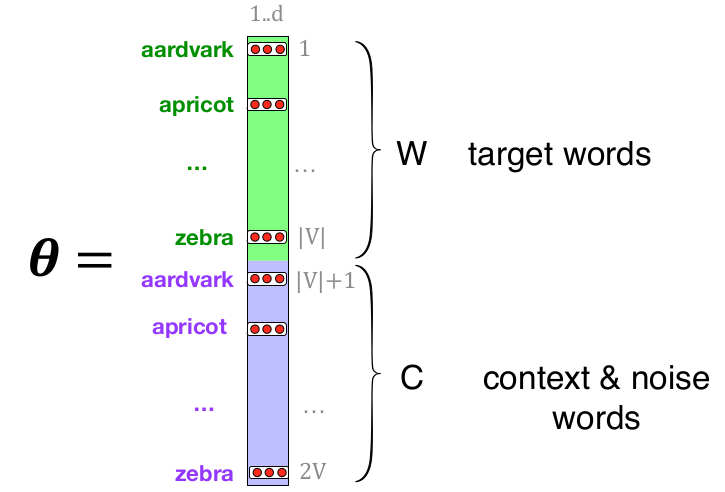
\includegraphics[scale=0.3]{img/word2vec_params.png}
      \end{center}
      Now given whatever sequence of $\pm c$ context words around a target, we will make the simplifying assumption that these words occur independently, and so the probability that a sequence of words $\mathbf{c}_{t-m:t+m}$ occur around $\mathbf{w}_t$ with window size $m$ is 
      \[\mu_{\boldsymbol{\theta}} (\mathbf{w}, \mathbf{c}_{t-m:t+m}) = \prod_{j=-m}^m \mu_{\boldsymbol{\theta}} (\mathbf{w}, \mathbf{c}_j)\]
      Now that we have our probabilistic model, we show how to generate our relevant training data. Consider the phrase 
      \[\texttt{... lemon, a [ tablespoon of apricot jam, a ] pinch ...}\]
      with $\texttt{apricot}$ as our target word. Just from this, we can generate 4 positive samples 
      \begin{align*}
          \mathbf{x}^{(1)}, y^{(1)} & = (\text{apricot}, \text{tablespoon}), 1 \\
          \mathbf{x}^{(2)}, y^{(2)} & = (\text{apricot}, \text{of}), 1 \\
          \mathbf{x}^{(3)}, y^{(3)} & = (\text{apricot}, \text{jam}), 1 \\
          \mathbf{x}^{(4)}, y^{(4)} & = (\text{apricot}, \text{a}), 1 
      \end{align*}
      where the words above would be in their one-hot encoded form. For training a binary classifier we need to have negative samples, too. Skip gram with negative sampling in fact uses more negative samples than positive ones (with the ration between them set by a parameter $R$). So for every positive sample, we pick a random noise word from the entire vocabulary, constrained not to be the target word $\mathbf{w}$. While this model could work with $R = 1$, it tends to perform better and is more stable if we have higher numbers, such as $R = 10, 15$. For example, if $R = 2$, then we would have 8 negative samples as such: 
      \begin{align*}
          \mathbf{x}^{(5)}, y^{(5)} & = (\text{apricot}, \text{aardvark}), 0 \\
          \mathbf{x}^{(6)}, y^{(6)} & = (\text{apricot}, \text{my}), 0 \\
          \mathbf{x}^{(7)}, y^{(7)} & = (\text{apricot}, \text{where}), 0 \\
          \mathbf{x}^{(8)}, y^{(8)} & = (\text{apricot}, \text{coaxial}), 0 \\
          \mathbf{x}^{(9)}, y^{(9)} & = (\text{apricot}, \text{seven}), 0 \\
          \mathbf{x}^{(10)}, y^{(10)} & = (\text{apricot}, \text{forever}), 0 \\
          \mathbf{x}^{(11)}, y^{(11)} & = (\text{apricot}, \text{dear}), 0 \\
          \mathbf{x}^{(12)}, y^{(12)} & = (\text{apricot}, \text{if}), 0 
      \end{align*}
      But these negative samples are not chosen randomly or according to counts. Rather, we sample them according to their \textbf{weighted unigram frequency}, usually of form 
      \[p_\alpha (c) = \frac{\mathrm{count}(c)^\alpha}{\sum_v \mathrm{count}(v)^\alpha}\]
      and setting $\alpha = 3/4$ gives the best results in practice, since it gives rare noise words slightly higher probability so most of the probability measure wouldn't be dominated by stop words like ``the". This is a probabilistic method, as there may be times when the negative sample actually occurs in the context, but 99.99\% of the time it will be a true negative sample. 

      To train the model, we should compute the likelihood of the entire training data. Given that we have our training data of form $(\mathbf{x}^{(n)}, y^{(n)}) = (\mathbf{w}^{(n)}, \mathbf{c}^{(n)}, y^{(n)})$ for $n = 1, \ldots, N$, our likelihood for the entire dataset is 
      \[L(\boldsymbol{\theta}) = \prod_{n=1}^N \mu_{\boldsymbol{\theta}} (\mathbf{w}^{(n)}, \mathbf{c}^{(n)})^{y^{(n)}} \big( 1 - \mu_{\boldsymbol{\theta}} (\mathbf{w}^{(n)}, \mathbf{c}^{(n)}) \big)^{1 - y^{(n)}} \]
      where we can take the negative average log and simplify further, but this is the extent that we will go for now. 
      \[- \ell (\boldsymbol{\theta}) = - \frac{1}{N} \sum_{n=1}^N y^{(n)} \log \big( \mu_{\boldsymbol{\theta}} (\mathbf{w}^{(n)}, \mathbf{c}^{(n)}) \big) + (1 - y^{(n)}) \, \log \big( 1 - \mu_{\boldsymbol{\theta}} (\mathbf{w}^{(n)} , \mathbf{c}^{(n)}) \big)\]
      Obviously we can use optimization techniques to minimize this w.r.t. $\boldsymbol{\theta}$. 

    \subsubsection{Continuous Bag of Words (CBOW)}

      To implement doc2vec, we utilize nltk for preprocessing and gensim to implement word2vec. 
      \begin{lstlisting}
        import string, nltk
        from nltk.corpus import brown
        from gensim.models import Word2Vec
         
        nltk.download("brown")

        # Preprocessing data to lowercase all words and remove single punctuation words
        document = brown.sents()

        data = []
        for sent in document:
          new_sent = []
          for word in sent:
            new_word = word.lower()
            if new_word[0] not in string.punctuation:
              new_sent.append(new_word)
          if len(new_sent) > 0:
            data.append(new_sent)
      \end{lstlisting}
      This data would be a list, with each element a list of tokens making up a sentence. For example, 
      \begin{lstlisting}
        # Total number of sentences/documents in corpus = 57158
        print(len(data))

        # Total number of words in first sentence/document = 22
        print(len(data[0]))

        # First list of tokens 
        print(data[0])
        # ['the', 'fulton', 'county', 'grand', 'jury', 'said', 'friday', 'an', 'investigation', 
        'of', "atlanta's", 'recent', 'primary', 'election', 'produced', 'no', 'evidence', 'that', 
        'any', 'irregularities', 'took', 'place']
      \end{lstlisting}
      Now we create the word2vec model and train it with the initializer containing the following parameters. Note that this is a stochastic process, and refer to the documentation to learn how we can make this deterministic. 
      \begin{lstlisting}
        model = Word2Vec(
            sentences = data,   # list of list of tokens 
            min_count = 5,      # Ignores all words with total frequency lower than this
            vector_size = 50,   # output vector dimensions
            window = 10,        # window of context words 
            epochs = 20,        # number of epochs trained over dataset 
            workers = 1,        # number of worker threads for multiprocessing
            sg = 0,             # 0 for CBOW, 1 for skip-gram
            hs = 0,             # 1 for hierarchical softmax, 0 for negative sampling
            negative = 5,       # num of negative samples per positive sample in skip-gram
            alpha = 0.025,      # training step
            min_alpha = 0.0001  # linearly decreases to this training step value 
        )
      \end{lstlisting}
      Now after training, this $\texttt{Word2Vec}$ object $\texttt{model}$ essentially has a dictionary with keys consisting of words in the corpus and values to be the embedding vectors. 
      \begin{lstlisting}
        print(model.wv["love"])

         [ 1.0745513  -1.8171308  -2.4329011  -0.3691842  -0.95292336 -0.54824775
          1.1184701  -1.2525641  -0.7875846  -3.7816436  -1.341159    2.6486464
         -0.30800238 -2.7417247   0.17696398 -2.9048784   1.621813    0.49121374
          0.4354661  -1.6528435  -2.4828649   0.4085583  -0.7043962   2.8490443
         -0.98837584  1.6951126  -1.607722    1.3588951  -0.03844598 -0.4779845
         -3.2942739   1.3696849   0.07875736  1.0799417  -1.6086684   0.6993245
          1.5824703   1.5176587   1.626068    1.7591808  -1.3893017  -2.4028397
         -0.36541265  0.71958435  2.0678997  -1.6587187   1.6821662  -3.3152702
         -1.6718794  -1.6396806 ]
      \end{lstlisting}

    \subsubsection{Intrinsic Word Vector Evaluation} 

      The word2vec performs quite well in preserving \textbf{semantic accuracy} (i.e. the meanings of the word). That is, it is true that the embedding $i \mapsto w_i$ often satisfies 
      \[w_{queen} = w_{\mathrm{king}} - w_{\mathrm{male}} + w_{\mathrm{female}}\]
      To quantify this analogy of $a : b = c : ?$, we want to find the word that is closest to $x_b - x_a + x_c$ in terms of cosine similarity. That is, we must find 
      \[d = \arg \max_i \frac{(x_b - x_a + x_c) \cdot x_i}{|| x_b - x_a + x_c ||}\]
      However, there is the possibility that this information is here, but it just may not be linear. Other very interesting relations, such as male/female, or even company/CEO, can be found. 
      \begin{center}
          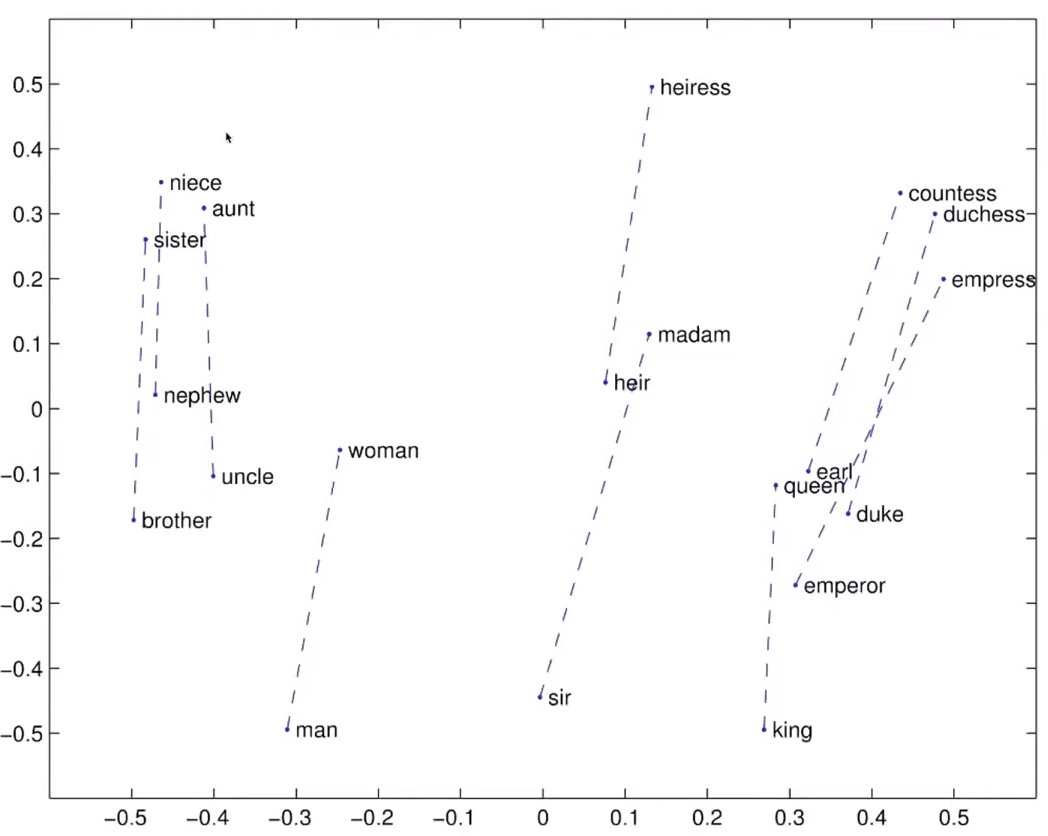
\includegraphics[scale=0.3]{img/GloVe_Visual.png}
      \end{center}
      Furthermore, we can capture \textbf{syntactic accuracy} (i.e. the grammar), as shown below using superlatives. 
      \begin{center}
          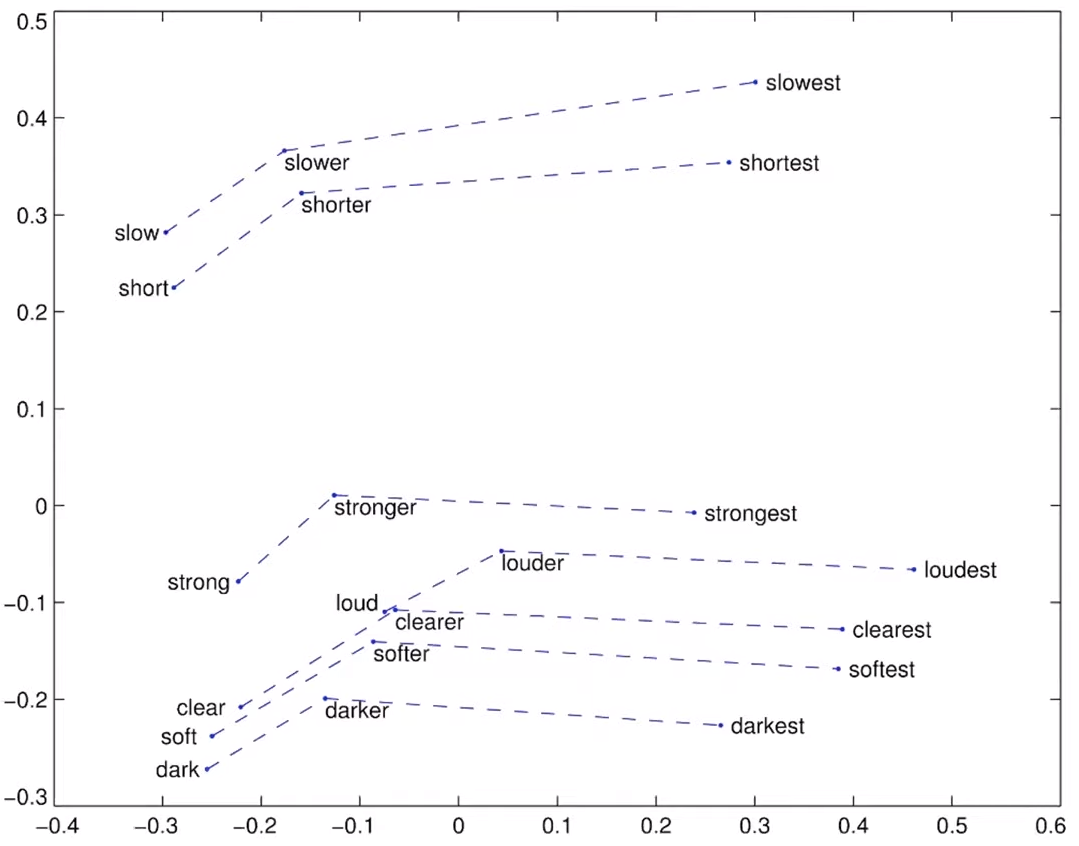
\includegraphics[scale=0.3]{img/syntactic.png}
      \end{center}

  \subsection{Doc2Vec}

    \subsubsection{Soft Cosine Measure}

    \subsubsection{Word Mover's Distance}

  \subsection{Global Vectors (GloVe)}

    The initial goal of GloVe was to connect the linear algebra based embeddings like LSA and COALS with the iterative, neural-updating models like skip-gram and CBOW. It seemed like linear algebra methods were superior since they have fast training times and have efficient use of statistics, but they were primarily used to capture word similarity. However, the NN models scales with corpus size, generate improve performance on other tasks, and can capture complex patterns beyond word similarity, though they have an inefficient use of statistics. 

    It is nice to encode the \textbf{meaning components} between words. That is, the concept of vector additions and subtractions work as an analogy (e.g. male to female, king to queen or verb to agent such as truck to driver). A new insight is that the \textit{ratios} of co-occurence probabilities can also encode the meaning components. Say that you want to capture the meaning component from solid to gas. We can take the co-occurence matrix of a document and compare the probabilities of certain words $x$ appearing around the context of ``ice" and ``steam." This gives us the matrix 
    \begin{center}
        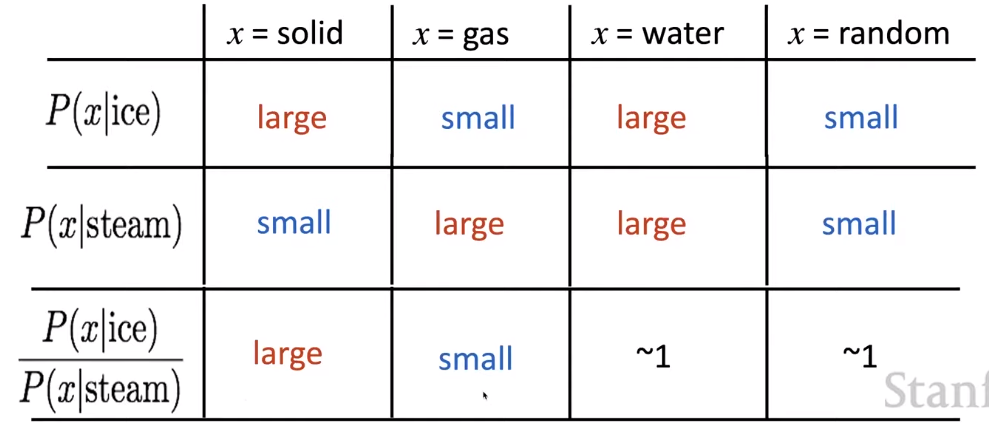
\includegraphics[scale=0.3]{img/solid_gas.png}
    \end{center}
    We would like to capture the ratios of co-occurence probabilities as linear meaning components in a word vector space. That is, the key property that we want is that the dot product of $w_i$ and $w_j$ represent the log probability of co-occurence. 

    It turned out that a log-bilinear model fits this well, by setting 
    \[w_i \cdot w_j = \log \mathbb{P}(i \mid j)\]
    with vector differences 
    \[w_x \cdot (w_a - w_b) = \log \frac{\mathbb{P}(x \mid a)}{\mathbb{P}(x \mid b)}\]
    The GloVe model wanted to unify the co-occurence model and the neural model, and so we wanted the dot product of two words $i$ and $j$ $w_i \mid w_j$ to be similar to the log of the co-occurence $\log{X_{ij}}$ (plus some bias), where $X$ is the matrix. Therefore, the entire loss function would be 
    \[J = \sum_{i, j = 1}^V f(X_{ij}) (w_i \cdot w_j + b_i + b_j - \log{X_{ij}})^2\]
    where we want our parameters $\boldsymbol{\theta} = \{ w_1, \ldots, w_V\}$ to be adjusted so that $w_i \cdot w_j$ is as close as possible to the log of the co-occurence matrix (with a bias term for both words). We also want to bound $X_{ij}$ with $f$ so that the loss isn't too dependent on a few very frequent words. 

    \subsubsection{Performance Comparison}

      Let us compare the semantic and syntactic performance of the embedding algorithms we know so far. As we can see in the table below, unscaled, raw-count SVD does terribly, but with proper scaling (SVD-S) or with COALS (SVD-L), we can get decent scores even without a neural network. CBOW and Skip Gram (SG) performs even better, but GloVe is the best performer, with the ideal embedding dimension being around 300. 
      \begin{center}
          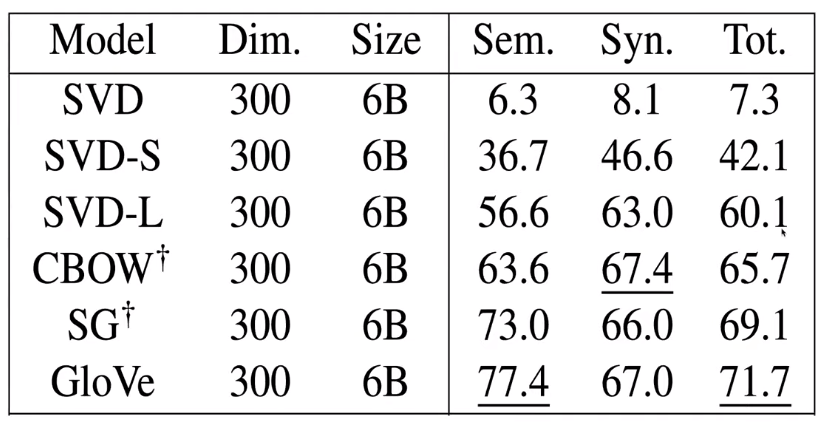
\includegraphics[scale=0.25]{img/comparison.png}
      \end{center}
      However, the author (and lecturer of the Stanford series I am working on) mentions that this outperformance may be due to having better data (Wikipedia is better than news text). 

  \subsection{Word Ambiguity}

    It is often the case that one word may have multiple meanings. For example, the word ``gay" may refer to homosexual or jolly. One simple solution is to train multiple embeddings for each definition of a word. The idea is that we cluster word windows around the words and retrain with each wod assigned to multiple different clusters, e.g. $\mathrm{bank}_1, \mathrm{bank}_2$, etc. 
    \begin{center}
        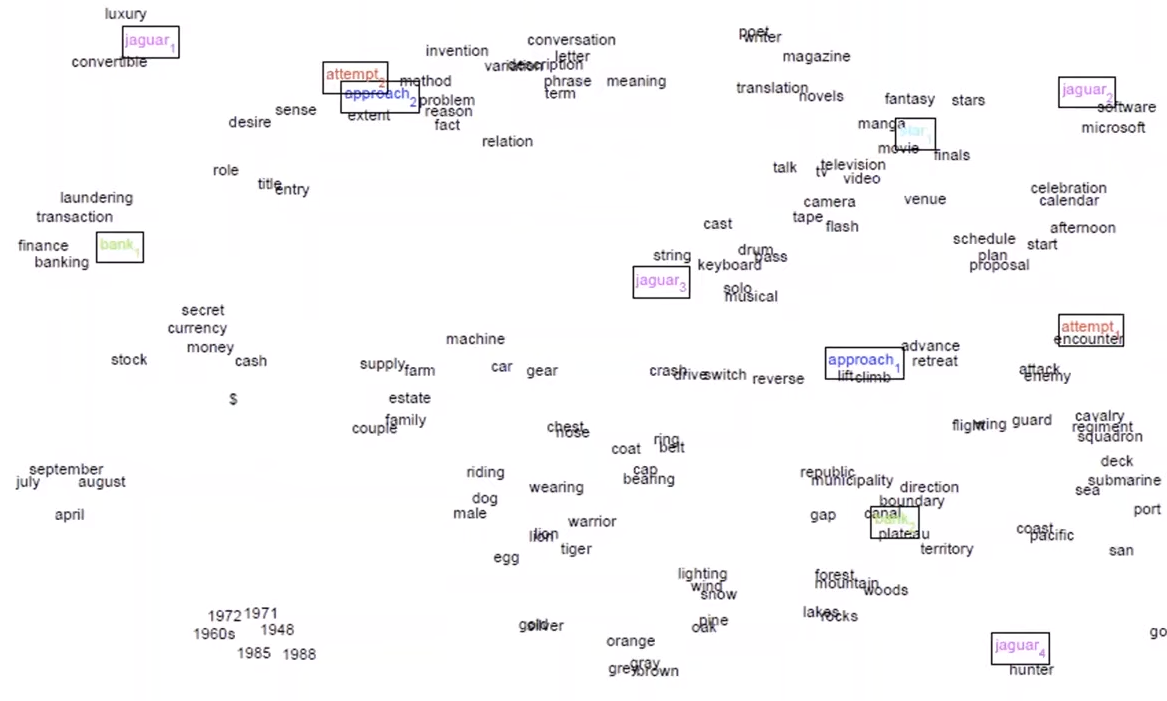
\includegraphics[scale=0.35]{img/ambiguity1.png}
    \end{center}
    This model works and aligns with our traditional sense of how these work, it tends to be imperfect since we're trying to refine our sense of a word into $k$ different parts. If we just keep the one-word one-embedding model, we find that different senses of the word reside in a ``linear superposition" (weighted sum) of embeddings of its sub-meanings. For example, 
    \[\text{bank} = \alpha_1 w_{\text{bank}_1} + \alpha_2 w_{\text{bank}_2} + \ldots + \alpha_k w_{\text{bank}_k}\]
    where $\alpha_i = \frac{f_i}{f_1 + \ldots f_k}$ for frequency $f$. This may look useless at first glance since we just have the average meaning of these vectors, but because of ideas from \textbf{sparse coding}, you can actually separate out the senses! This is possible because in high-dimensional vector spaces, things tend to be extremely sparse. 

\section{Classical Learning Approaches}

  Some include sentiment analysis, and dependency structure. 

  \subsection{Logistic Regression}

  \subsection{Latent Dirichlet Allocation (LDA)}

\section{Sequence Tagging and Dependency Parsing}

  If we have a good word embedding model parts of speech or named entity recognition would be much easier. However, we will also regard it as a problem in its own right. 

  Dependency parsing is a natural language processing (NLP) technique that analyzes the grammatical structure of a sentence by determining the relationships between words. It aims to identify the syntactic dependencies among words and represent them as a directed graph, known as a dependency tree.

  In dependency parsing, each word in a sentence is assigned a grammatical role (such as subject, object, modifier, etc.) and linked to its corresponding head word, which governs or controls it. The relationships between words are represented as labeled directed edges, where the head word is the parent node, and the dependent word is the child node.

  For example, consider the sentence: "John eats an apple." In dependency parsing, the word "eats" would be the head word, and "John" and "apple" would be its dependents. The word "eats" would have a dependency relation of "subject" with "John" and "object" with "apple." This information can be represented as a dependency tree, where "eats" is the root, "John" is connected to "eats" with a subject edge, and "apple" is connected to "eats" with an object edge.

  Dependency parsing has various applications in NLP, including syntactic analysis, information extraction, machine translation, sentiment analysis, and question answering. It helps in understanding the structure of a sentence, resolving ambiguities, and enabling more sophisticated language processing tasks. Dependency parsers can be trained using machine learning techniques, such as supervised learning or transition-based parsing algorithms, using annotated dependency treebanks.

  Sentiment classification - Logistic, MLPs, RNNs (element-wise max or mean of all hidden states, Lec 6 34:17) 
  Sequence Tagging - HMM, CRF, MLPs, RNNs
  Dependency Parsing - 
  Language Encoder Module - Question Answering, Machine Translation 
  Text Generation - i.e. RNN-LMs

\section{Basic Language Models}

  Unlike classification problems, \textbf{language modeling} refers to the task of predicting upcoming words from prior word context. That is, given a string of words $w_1, \ldots, w_{t-1}$, we want to provide a conditional probability distribution of 
  \[\mathbb{P}(w_t \mid w_{t-1}, \ldots, w_1 )\]

  \subsection{N Gram Model}

    An N-gram model basically models this as a giant Markov chain, which approximates the probability distribution of the next word as dependent on only the last $t-1$ words.
    \[\mathbb{P}(w_t \mid w_{t-1}, \ldots, w_{1}) \approx \mathbb{P}( w_t \mid w_{t-1}, \ldots, w_{t - N + 1}) = \frac{\mathbb{P}(w_t, w_{t-1}, \ldots, w_{t-N+1})}{\mathbb{P}(w_{t-1}, \ldots, w_{t-N+1})}\]
    In order to calculate this probability, we literally just count them in some large corpus of text. 
    In order to construct such as model there are two functions that will be helpful: NLTK's $\texttt{word\_tokenize}$ and $\texttt{ngrams}$ methods. 
    \begin{lstlisting}
    from nltk.tokenize import word_tokenize 
    from nltk import ngrams 

    sentence = "I love data science and machine learning."
    tokens = word_tokenize(sentence) 
    # ['I', 'love', 'data', 'science', 'and', 'machine', 'learning', '.']

    grams = list(ngrams(tokens, 3, 
                        pad_left=True, 
                        pad_right=True, 
                        left_pad_symbol='<s>', 
                        right_pad_symbol='</s>'
                        ) 
                 )
    # [('<s>', '<s>', 'I'), ('<s>', 'I', 'love'), ('I', 'love', 'data'), ('love', 'data', 
    # 'science'), ('data', 'science', 'and'), ('science', 'and', 'machine'), ('and', 
    # 'machine', 'learning'), ('machine', 'learning', '.'), ('learning', '.', '</s>'), ('.', 
    # '</s>', '</s>')]
    \end{lstlisting}
    Now this works for only one sentence, so if we take in a document with many sentences, we would like to construct a data structure that maps from the set of $N-1$ previous words to the next word. From here we will create a very crude N-gram model. 
    \begin{lstlisting}
    import random, time
    from nltk.tokenize import word_tokenize, sent_tokenize
    from nltk import ngrams

    class NgramModel(object): 
        
        def __init__(self, N:int, path:str): 
            
            now = time.time()
            
            self.N = N 
            self.context = {}
            
            with open(path, 'r') as f:
                sentences = sent_tokenize(f.read()) 
                
                for sentence in sentences: 
                    tokens = word_tokenize(sentence)
                
                    grams = ngrams(tokens, N, 
                        pad_left=True, 
                        pad_right=True, 
                        left_pad_symbol='<s>', 
                        right_pad_symbol='</s>'
                        )
                    
                    for tup in grams: 
                        prev_words = tup[:-1] 
                        next_word = tup[-1]
                        if prev_words in self.context: 
                            self.context[prev_words].append(next_word)
                        else: 
                            self.context[prev_words] = [next_word]
                            
                    # finally add the (</s>, </s>) -> <s> | (</s>, <s>) -> <s> ...
                    final = ["</s>"] * (self.N - 1) 
                    for _ in range(self.N - 1): 
                        self.context[tuple(final)] = ["<s>"]
                        final.pop(0) 
                        final.append("<s>")
                            
            print(f"Time Taken to Create Model : {time.time() - now}")
                    
    \end{lstlisting}
    Then we can put in our helper functions for generating text. 
    \begin{lstlisting}
        def next_rand_word(self, prev_words:tuple): 
                return random.choice(self.context[prev_words])
            
            def generate_text(self, n_words = 50): 
                
                result = []
                prev = ["<s>"] * (self.N - 1)
                
                step = 0
                while step < n_words: 
                    next = self.next_rand_word(tuple(prev)) 
                    
                    if next not in ["<s>", "</s>"]: 
                        result.append(next) 
                        step += 1
                    
                    prev.pop(0) 
                    
                    prev.append(next)
        
                print(" ".join(result))
    \end{lstlisting}
    Now running it on Mary Shelly's Frankenstein gives the following: 
    \begin{lstlisting}
    m = NgramModel(5, "/home/mbahng/Desktop/Chatbot/Frankenstein.txt")    
    m.generate\_text(500)

    Time Taken to Create Model : 0.5771486759185791
    As I sat , a train of reflection occurred to me which led me to consider the effects of 
    what I was now doing . Reserve on such a point would be not only useless , but draw down 
    treble misery on us all. " I trembled violently at his exordium , and my father reposed .
    My abhorrence of this fiend can not be conceived . As I spoke , rage sparkled in my eyes 
    ; the females were flying and the enraged Felix tearing me from his father , to whose 
    knees I clung , in a transport
    \end{lstlisting}

    However, we end with some problems of this model. Remember that we must compute 
    \begin{equation}
      \mathbb{P}(w_t \mid w_{t-1}, \ldots, w_{1}) \approx \mathbb{P}( w_t \mid w_{t-1}, \ldots, w_{t - N + 1}) = \frac{\mathbb{P}(w_t, w_{t-1}, \ldots, w_{t-N+1})}{\mathbb{P}(w_{t-1}, \ldots, w_{t-N+1})}
    \end{equation}
    at every time step.
    \begin{enumerate}
        \item One sparsity problem is that we will compute $\mathbb{P}(w_t, w_{t-1}, \ldots, w_{t-N+1}) = 0$ since $w_t$ never followed after the phrase $w_{t-N+1}, \ldots, w_{t-1}$, which may be inaccurate if $w$ is indeed used often outside the context. This can be fixed by \textbf{smoothing}, i.e. adding a small $\delta$ to the count for every $w \in \mathcal{V}$. 
        
        \item If the denominator itself doesn't occur at all in the text, then its probability will be $0$! Therefore, we can't calculate the probability for \textit{any} $w_t$! What we can do is just condition on a shorter phrase with the following approximate, which is called \textbf{backoff}. 
        \begin{equation}
          \mathbb{P}( w_t \mid \underbrace{w_{t - N + 1}, \ldots, w_{t-1}}_{N-1 \text{ words}}) \approx \mathbb{P}( w_t \mid \underbrace{w_{t - N + 2}, \ldots, w_{t-1}}_{N-2 \text{ words}})
        \end{equation}

        \item It may require a lot of memory to store these giant dictionaries containing millions or billions of elements. This is not scalable. 
    \end{enumerate}
    Note that increasing $N$ makes the sparsity problems worse, and typically we can't have $N$ bigger than $5$. 

  \subsection{Fixed Window Neural Model}

    Neural language models have many advantages over the n-gram language. Compared to n-gram models, neural language models can handle much longer histories, can generalize better over contexts of similar words, and are more accurate at word prediction. On the other hand, neural net language models are much more complex, are slower and need more energy to train, and are less interpretable than n-gram models, so for many 
    especially smaller) tasks an n-gram language model is still the right tool. 

    A neural language model is similar to an n-gram as it takes as input at time $t$ a representation of some number of previous words $(w_{t-1}, w_{t-2}, \ldots$) and outputs a probability distribution of $w_t$ over some possible set of words. We also estimate based on a constant number of $N$ previous words: 
    \[\mathbb{P}(w_t \mid w_1, \ldots, w_{t-1}) \approx \mathbb{P}( w_t \mid w_{t - N + 1}, \ldots, w_{t-1})\]
    If you are familiar with neural nets, then with word embeddings, you should have a good idea of how this can be implemented. Another advantage of using embeddings is that neural nets can generalize better to unseen data. For example, if we have never seen the word ``dog" but have seen ``cat," we can use the fact that the two words have similar embeddings to predict the next words after ``dog," whereas in a vanilla n-gram model we don't know. 

    Now given a corpus with total vocabulary $\mathcal{V}$ consisting of words $v_i$ for $i = 1, \ldots, |\mathcal{V}|$, we can one-hot encode all the vectors $\mathbf{v}_i \mapsto \mathbf{x}_i$, which are the standard vectors. We can train a $d$-dimensional embedding on the words (e.g. doc2vec) which results in a $d \times |\mathcal{V}|$ \textbf{embedding matrix} $\mathbf{E}$ of form 
    \[\begin{bmatrix} | & \ldots & | \\ \mathbf{E}_1 & \ldots & \mathbf{E}_{|\mathcal{V}|} \\ | & \ldots & | \end{bmatrix}\]
    where the $i$th column $\mathbf{E}_i$ represents the embedding of $v_i$. This makes it easy to map the one-hot vectors since $\mathbf{E}_i = \mathbf{E} \mathbf{x}_i$. Now, just like the n-gram model, we must use the previous $N$ words to predict the next word. Therefore, if we have words $v_{t - N}, \ldots, v_{t-1}$, we can calculate their embeddings and use these vectors to train our model. The forward pass of the multilayer perceptron is outlined below: 
    \begin{enumerate}
        \item Given the $N$ previous words $\mathbf{x}_{i_{t-N}}, \ldots, \mathbf{x}_{i_{t-1}}$, take their embedding $\mathbf{E} \mathbf{x}_{i_{t-N}}$ and vertically stack them on top of each other to create a $Nd$-dimensional vector. 
        \[\mathbf{e} = \big[ \mathbf{E} \mathbf{x}_{i_{t-N}} ; \ldots ; \mathbf{E} \mathbf{x}_{i_{t-1}} \big] \]

        \item We input this through a hidden layer by multiplying it by $\mathbf{W}^{[1]}$ (and adding a bias term) and then through an activation layer $\boldsymbol{\sigma}^{[1]}$. This is done $L$ times for a $L$-layer MLP: 
        \[\mathbf{h}_{\boldsymbol{\theta}} (\mathbf{e}) = \boldsymbol{\sigma}^{[L]} \circ \mathbf{W}^{[L]} \circ \boldsymbol{\sigma}^{[L-1]} \circ \mathbf{W}^{[L-1]} \circ \cdots \circ \boldsymbol{\sigma}^{[1]} \circ \mathbf{W}^{[1]} (\mathbf{e})\]

        \item We multiply by the final linear map $\mathbf{U}: \mathbb{R}^{N^{[L]}} \rightarrow \mathbb{R}^{|\mathcal{V}|}$ and then apply the softmax activation function to get a vector of probabilities. 
        \[\hat{\mathbf{y}} = \mathrm{softmax} \big( \mathbf{U} \mathbf{h}_{\boldsymbol{\theta}} (\mathbf{e}) + \mathbf{b}_\mathbf{U} \big) \]
    \end{enumerate}

    Even though this does eliminate all the sparsity problems of an n-gram model, there are some remaining problems. 
    \begin{enumerate}
        \item First, while we can always increase the window size, it can never be large enough. That is, there may always be some dependencies that we must watch out for that is beyond the window length of the neural model. 
        \item Furthermore, words in different positions are multiplied by completely different weights in $W$, and so there is no symmetry in how the inputs are processed. 
    \end{enumerate}
    Therefore, we need a neural architecture that can process inputs of any length, i.e. a RNN. 

  \subsection{Vanilla RNNs}

    The recurrent neural network can process any length input, the model size does not increase for longer input text, and the same weights are applied on every timestep, so there is symmetry in how inputs are processed. However, the computation can be slow since this is sequential by definition. We can take the corpus, add the START and END tokens in it, and train the RNN with minibatch SGD by sampling 32 to 64 sentences from the corpus and computing the gradient of the cross-entropy loss with teacher forcing. Then, we can simply input in the START token as the first input $\mathbf{x}_1$, which will generate the next word that we set as the second sequential input $\hat{\mathbf{y}}_1 = \mathbf{x}_2$. 

    \subsubsection{Bidirectional RNNs}

      For problems in, say sentiment classification, the context of not just the previous words, but also the future words, may be relevant to determining the sentiment. For example, take the following sentence: 
      \begin{lstlisting}
          The movie was terribly exciting. 
      \end{lstlisting}
      The terribly part might be interpreted as a negative sentiment, when it is actually being used as an adjective to describe exciting. Therefore, we want to use bidirectional or multilayer RNNs to capture the entire sentence before outputting anything. 

      Note that birdirectional RNNs are only applicable if you have access to the entire input sequence. You can't use them in language modeling since in LM you onl have \textit{left} context available. If you do have the entire input sequence, bidirectionality is powerful and you should use it by defaut. For example, BERT (Bidirectional Encoder Representations from Transformers) is a powerful pretrained contextual representation system built on bidirectionality. 

    \subsubsection{Perplexity Evaluation} 

      The standard evaluation metric for language models is \textbf{perplexity}, which has a very nice intuitive definition behind it. Assume that a stream of words $\mathbf{x}_1, \ldots, \mathbf{x}_T$ is generated by the model. We can calculate the probability of this sentence being generated by taking the product of conditional probabilities 
      \[\prod_{t=1}^T \mathbb{P}_{\mathrm{LM}} (\mathbf{x}_{t+1} \mid \mathbf{x}_t, \ldots, \mathbf{x}_1)\]
      This measure would mean that longer sentences would have less probability assigned to them just because they are shorter, so we must take the geometric mean of this. 
      \[\bigg( \prod_{t=1}^T \mathbb{P}_{\mathrm{LM}} (\mathbf{x}_{t+1} \mid \mathbf{x}_t, \ldots, \mathbf{x}_1) \bigg)^{1/T}\]
      If this number is high, then this means that the probability of this sentence being generated is also high and therefore this language model is good. If we consider all the conditional distributions to be very sharply peaked around one word, then there is not much variability on how the sentence is generated. However, if all the conditional distributions are generally uniform, then there is a lot of variability in the sentence generation. In fact, this is closely related to the concept of entropy. In fact, a uniform conditional probability distribution for all possible cases would correspond to both maximum entropy and minimum probability since (if $V$ is the size of the vocabulary)
      \[\bigg( \prod_{t=1}^T \mathbb{P}_{\mathrm{LM}} (\mathbf{x}_{t+1} \mid \mathbf{x}_t, \ldots, \mathbf{x}_1) \bigg)^{1/T} = \bigg( \prod_{t=1}^T \frac{1}{V} \bigg)^{1/T} = \frac{1}{V}\]
      Finally, perplexity itself is just defined as the inverse of this probability, so lower perplexity is better. 
      \[\prod_{t=1}^T \bigg( \frac{1}{\mathbb{P}_{\mathrm{LM}} (\mathbf{x}_{t+1} \mid \mathbf{x}_t, \ldots, \mathbf{x}_1)} \bigg)^{1/T}\]
      It can also be seen as equivalent to the cross-entropy loss. Of course, perplexity is a stochastic variable, but on average, the worst possible perplexity is $V$ itself, which may be very high if the corpus is large. Some common perplexities are shown below, with later rows representing increasingly complex RNNS. 
      \begin{center}
          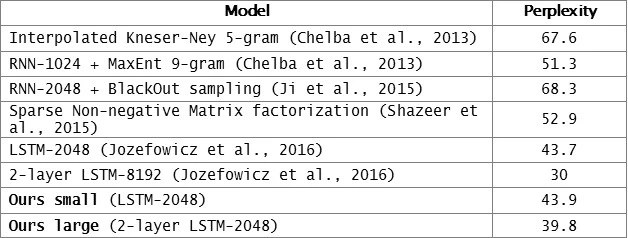
\includegraphics[scale=0.5]{img/perplexity.png}
      \end{center}

    \subsubsection{BLEU}

      The \textbf{Bilingual Evaluation Understudy (BLEU)} compares the machine-written translation to one or several human-written translations, and computes a similarity score based on 
      \begin{enumerate}
          \item n-gram precision (usually for 1, 2, 3, 4-grams) 
          \item plus a penalty for too-short system translations. 
      \end{enumerate}
      It is useful but imperfect since there are many valid ways to translate a sentence. Therefore, a good translation can get a poor BLEU performance because it has low n-gram overlap with the human translation. 

  \subsection{LSTMs}

    However, the problem of vanishing (and exploding) gradients render the vanilla RNN practically infeasible. Due to the exponential memory loss of the RNN, these models have a hard time modelling long-term dependencies between words. For example, take a look at the following sentence, with a blank at the end where the RNN-LM must fill out. 
    \begin{lstlisting}
        When she tried to print her tickets, she found that the printer was out of toner. 
        She went to the stationery store to buy more toner. It was very overpriced. After 
        installing the toner into the printer, she finally printed her \_\_\_\_\_. 
    \end{lstlisting}
    In here, the RNN would have to remember the ``tickets" on the 7th word all the way up to the end. Therefore, we introduce the LSTM model. 
    \begin{center}

    \end{center}

\section{Encoder-Decoder Machine Translation Models}

    Let us first focus on the problem of language translation. \textbf{Machine Translation (MT)} is the task of translating a sentence $x$ from one language (the \textbf{source language}) to a sentence $y$ in another language (the \textbf{target language}). 
    \begin{lstlisting}
      x:   L'homme est ne libre, et partout il est dans les fers 
      y:   Man is born free, but everywhere he is in chains 
    \end{lstlisting}

  \subsection{Statistical Machine Translation}

    Machine translation first started in the 1950s when, following the computer's extreme success in many problems, the U.S. decided to use them for translating Russian to English. This was a much harder problem to solve, but in the 1990s to 2010s, this idea was reborn again in the form of \textbf{statistical machine translation (SMT)}. The idea was to learn a probabilistic model from the data. That is, given a French sentence $x$, we want to find the best English sentence $y$, which we can use Bayes rule to break this down into two components to be learned separately.  
    \[\arg \max_{y} \mathbb{P}(y \mid x) = \arg \max_y \mathbb{P}(x \mid y) \mathbb{P}(y) \]
    \begin{enumerate}
        \item The left hand distribution $\mathbf{P}(x \mid y)$ models how words and phrases should be translated (\textit{fidelity}), which are learned from parallel data (data of paired English/French sentences). 
        \item The right distribution $\mathbf{P}(y)$ models how to write good English (\textit{fluency}), which is learnt from monolingual data. 
    \end{enumerate}
    This obviously requires a lot of parallel data, which can be found in international conferences and such. To go into the details, we want to learn the translation model $\mathbb{P}(x \mid y)$ from the parallel corpus by introducing a latent variable $a$ into the model $\mathbf{P}(x, a \mid y)$, where $a$ is called the \textbf{alignment}. This represents the word-level correspondence between source sentence $x$ and target sentence $y$. 

    \begin{center}
      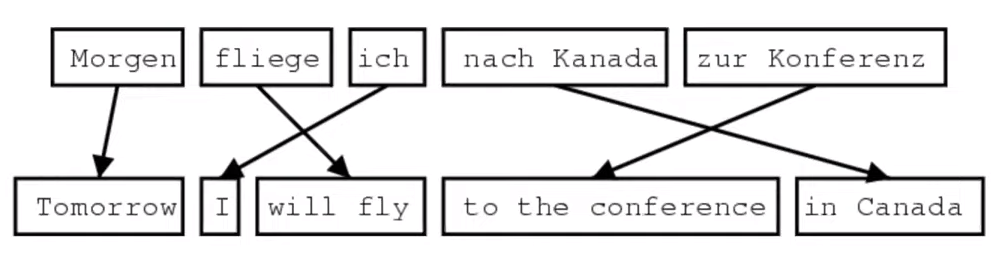
\includegraphics[scale=0.3]{img/alignment.png}
    \end{center}

    Alignment refers to the correspondence between particular sets of words in the translated sentence pair. Note that it is not as simple as just connecting two individual words, as some words may need to be translated into a phrase, vice versa, or some phrases/words may have no counterpart at all! Not to mention we also need to account for words with multiple meanings. From this, it is clear that alignment can be extremely complex. Essentially, the distributions are learned as a combination of many factors, including the probability of particular words aligning, and the alignments are also learned (they are not labeled in the data!) using special learning algorithms like Expectation-Maximization (EM). 

    During this time period, SMT was a huge field, with extremely complex SOTA systems with hundreds of details. These systems had many separately-designed subcomponents and required a lot of feature engineering (designing features to capture particular language phenomena). It also required compiling and maintaining extra resources, like tables or equivalent phrases, necessitating a lot of human effort. 

  \subsection{Neural Machine Translation}

    Post-2010, \textbf{neural machine translation (NMT)} models, which performs machine translation with a single end-to-end neural network, have become SOTA. We can use a \textbf{sequence-to-sequence} (\textbf{seq2seq}) encoder-decoder model with some pretrained word embeddings to learn the translation. This seq2seq is an example of a conditional language model, since it is predicting the next word of the target sentence $y$ by conditioning on the source sentence $x$. It directly calculates $\mathbb{P}(y \mid x)$ by expanding it as 
    \[\mathbb{P}(y \mid x) = \mathbb{P}(y_1 \mid x) \, \mathbb{P}(y_2 \mid y_1, x) \, \ldots \mathbb{P}(y_T \mid y_1, \ldots, y_{T-1}, x)\]

  \subsection{Decoding Schemes}

    Note that every sequential output of the decoder takes the output of the final layer hidden cell, multiplies it by some matrix, and finally invokes some activation function on it. Consider a classification problem where we have $V$ classes, with a linear map mapping to $\mathbb{R}^{V}$, followed by a softmax activation. It seems most natural to choose the class that has the maximum probability from the softmax, but this greedy algorithmic approach may not be ideal since we may be giving up long term benefits for short term ones. What we really want to do find the sequence $y$ that maximizes 
    \[\mathbb{P}(y \mid x) = \prod_{t=1}^T \mathbb{P}( y_t \mid y_{1}, \ldots, y_{t-1}, x)\]
    Clearly, computing the joint probability distribution over all sequences is too expensive, so we can do \textbf{beam search decoding}. The main idea is that on each step of the decoder, we keep track of the $k$ (in practice around 5 to 10) most probable partial outputs. For example in the case of machine translation, given a beam size of $k = 2$, we can keep track of the (log) probabilities of the sequences and only keep track of the top $2$. 
    \begin{enumerate}
        \item Given the START token, say that the $k$ most probable next words were ``he" ($-0.7$) and ``I" ($-0.9$). 
        \begin{center}
            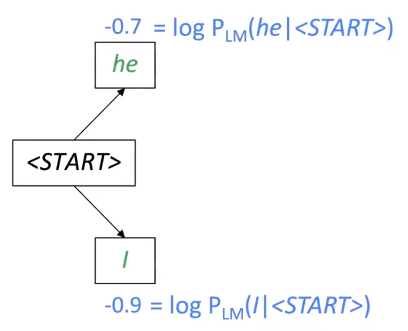
\includegraphics[scale=0.3]{img/beam1.png}
        \end{center}

        \item Now we look at the two most likely next words for each of ``he" and ``I" and out of the four possibilities, we compute the two most likely ones, which is ``he hit" ($-1.7$) and ``I was" ($-1.6$). 
        \begin{center}
            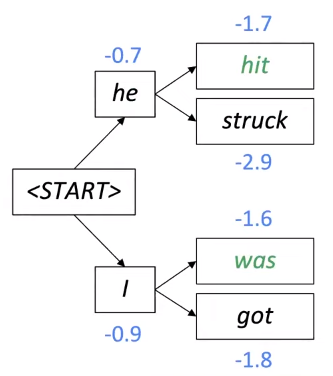
\includegraphics[scale=0.3]{img/beam2.png}
        \end{center}

        \item We keep track of ``he hit" and ``I was" and find the two most likely next words for each, leading us to another four possibilities. We compute the two most likely ones, which is ``he hit me" ($-2.5$) and ``he hit a" ($-2.8$). 
        \begin{center}
            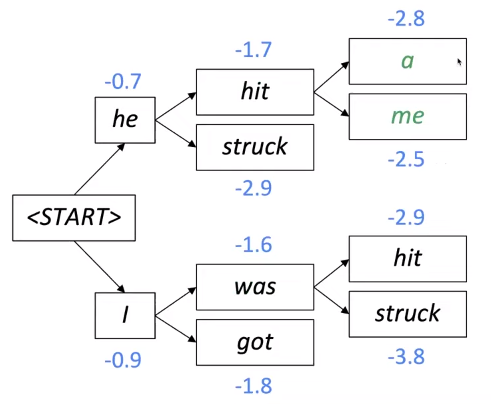
\includegraphics[scale=0.3]{img/beam3.png}
        \end{center}

        \item We keep repeating this.  
        \begin{center}
            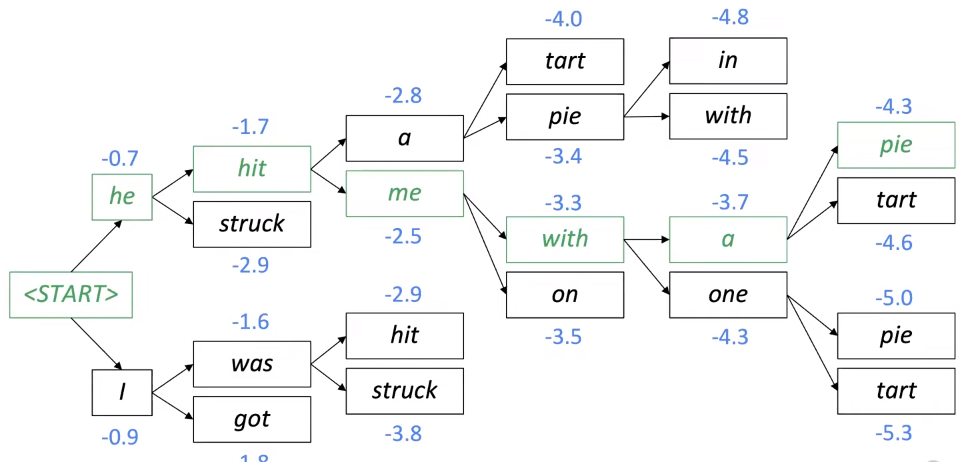
\includegraphics[scale=0.3]{img/beam4.png}
        \end{center}
    \end{enumerate}
    One more condition to mention is when to stop generating words. In greedy decoding, we usually decode until the model produces an END token. In beam search decoding, different hypotheses may produce END tokens on different timestamps, and so every time we have a complete hypothesis, we can place it aside and continue exploring other hypotheses via beam search. We can continue beam searching until we reach some predetermined cutoff timestep $T$ or we have at least $n$ completed hypotheses (where $n$ is also some predetermined cutoff). We have a slight problem that longer hypotheses will have lower log probabilities, so we can choose the best output sequence by taking the average log probabilities (which corresponds to the geometric mean of the probabilities). 
    \[\mathrm{score}(y_{t+1}, \ldots, y_T) = \frac{1}{T-t} \log \mathbb{P}_{LM} (y_1, \ldots, y_t \mid x) = \frac{1}{T-t} \sum_{k=t+1}^T \log \mathbb{P}_{LM} ( y_k \mid y_{t+1}, \ldots, y_{k-1}, x) \]

  \subsection{Attention}

    A huge issue with the sequence-to-sequence model is the \textbf{bottleneck problem}. The encoder encodes the input sentence into a single latent vector at the end, and this one vector needs to capture \textit{all information} about the source sentence. Clearly, if this vector is not large enough, we have too little bandwidth to capture this information, resulting in an information bottleneck. 

    The idea of \textbf{attention} provides a solution to this bottleneck problem. Basically, we want to establish connections from the decoder to not just the last hidden state of the encoder, but to all of its nodes. Each encoder node represents some information about each word, and by taking some weighted sum of these nodes, we can choose which one to put this attention on. The specific steps are listed: 
    \begin{enumerate}
        \item We have encoder hidden states $\mathbf{h}_1, \ldots, \mathbf{h}_N \in \mathbb{R}^h$. 
        \item On timestep $t$, we have the decoder hidden state $\mathbf{s}_t \in \mathbb{R}^h$.  
        \item We get the attention scores $\mathbf{e}^t$ for this step by computing 
        \[\mathbf{e}^t = \big( \mathbf{s}_t^T \mathbf{h}_1 , \ldots, \mathbf{s}_t^T \mathbf{h}_N \big) \in \mathbb{R}^N\]
        \item We take its softmax to get the \textbf{attention distribution} $\boldsymbol{\alpha}^t$ for this step (a discrete probability distribution) 
        \[\boldsymbol{\alpha} = \mathrm{softmax} (\mathbf{e}^t) \in \mathbb{R}^N\]

        \item We use $\boldsymbol{\alpha}^t$ to take a weighted sum of the encoder hidden states to get the attention output $\mathbf{a}_t$ 
        \[\mathbf{a}_t = \sum_{i=1}^N \alpha_i^t \mathbf{h}_i \in \mathbb{R}^h\]

        \item We concatenate the attention output $\mathbf{a}_t$ with the decoder hidden state $\mathbf{s}_t$ and proceed as in the non-attention seq2seq model. 
        \[[\mathbf{a}_t ; \mathbf{s}_t ] \in \mathbb{R}^{2h}\]
    \end{enumerate}

\section{Transformer Based Models}

\bibliography{./bibfile}
\bibliographystyle{alpha}

\end{document}

